%   SETUP%
\documentclass[a4paper,11pt,oneside,titlepage]{book}
\usepackage[T1]{fontenc}		% Codifica dei font; T1 codifica di output dell'italiano e di lingue occidentali
\usepackage[utf8]{inputenc}		% Codifica degli input; abilita l'utilizzo di caratteri accentati
\usepackage[italian]{babel}		% Set the languages; the last one is the main language
\usepackage{geometry}			% Allow to change the margin
\usepackage{setspace}			% Allow to change the interline with \begin{onehalfspaceng} ecc.
\usepackage{fancyhdr}			% Fancy style for page layout
\usepackage{afterpage} 			% Allow to load blank pages with the command '\afterpage{\null\thispagestyle{empty}\clearpage}' 
\usepackage{hyperref}			% Crea collegamenti ipertestuali rendendo cliccabili i riferimenti
\usepackage{url}
\usepackage{color}			% Allow to use colors
\usepackage{xcolor}			% manage colors
\usepackage{enumerate}			% Numbered lists
\usepackage{enumitem}			% Allow to manage the style of the list
\usepackage{graphicx}			% Images
\usepackage{epstopdf}			% allows to convert eps images to pdf for use with pdflatex
\usepackage{pstool}			% Allows to use psfrag with pdflatex (no latex compiler needed)
\usepackage{psfrag}
%\usepackage[normal]{subfigure}		% manage subfigures
\usepackage{subfig}		% manage subfigures
\usepackage{array}			% Tables
\usepackage{tabularx}			% allow to set the width of the whole table
\usepackage[bottom]{footmisc}		% To attach footnote at the end of the page
\usepackage{booktabs}			% is a must for professional-looking layout
\usepackage{longtable}			% is very popular for multi-page tables
\usepackage{caption}			% Captions
\usepackage{float}			% Manage float objects (image, table, ecc.)
\usepackage{rotating}			% permette di ruotare immagini, tabelle, ecc. di 90° o di 270°
\usepackage{rotfloat}			% costruisce un ponte tra i pacchetti float e rotating
\usepackage{amsmath} 			% Equations
\usepackage{amssymb}			% Mathematical Symbols
\usepackage{cancel}                     % Simplification Cancellation
\usepackage{mleftright}
\usepackage{listings}                   % Codes
\definecolor{lstgreen}{rgb}{0,0.6,0}
\definecolor{lstgray}{rgb}{0.5,0.5,0.5}
\definecolor{lstmauve}{rgb}{0.58,0,0.82}
\lstset{ %
  backgroundcolor=\color{white},   % choose the background color
  basicstyle=\footnotesize,        % size of fonts used for the code
  breaklines=true,                 % automatic line breaking only at whitespace
  captionpos=b,                    % sets the caption-position to bottom
  commentstyle=\color{lstgreen},    % comment style
  escapeinside={\%*}{*)},          % if you want to add LaTeX within your code
  keywordstyle=\color{blue},       % keyword style
  stringstyle=\color{lstmauve},     % string literal style
}
%\usepackage{vector}  			% Allows "\bvec{}" and "\buvec{}" for "blackboard" style bold vectors in maths
\usepackage[swapnames,norules,nouppercase]{frontespizio}
%\usepackage[intoc]{nomencl}	% disabled: loads KOMA tocbasic, which errors with caption on TeX Live 2025
\usepackage[acronym,toc,nomain,nopostdot,nonumberlist]{glossaries}
\usepackage[square, numbers, comma, sort&compress]{natbib}
\usepackage{verbatim}                   % Needed for the "comment" environment to make LaTeX comments
\usepackage{wrapfig}                 % Per inserire le figure contornate da testo
\usepackage{blindtext}
\geometry{a4paper,top=2.5cm,bottom=2.5cm,left=2cm,right=2cm,heightrounded,bindingoffset=5mm,headheight=13.6pt}
% -------------------------------------- Line-spacing --------------------------------------- %
\linespread{1.2} 
%\linespread{1.5} 
%\linespread{2} 
%\raggedbottom % disattiva lo 'stiracchiamento' del testo; va a favore di spazio bianco a fondo pagina
% ---------------------------------------- Numeration --------------------------------------- %
%\setcounter{secnumdepth}{3} % set the enumeration of the sections
%\setcounter{tocdepth}{3}    % set the enumeration of the sections in the table of contents
%--------------------------------------- Page layout -----------------------------------------%
%\pagestyle{fancy}                       % definisce lo stile di pagina aprendo la strada al pacchetto fancyhdr
%\renewcommand{\chaptermark}[1]{\markright{\chaptername\ \thechapter.\ #1}{}}    % ridefinisce la macro \rightmark per i capitoli
%\renewcommand{\sectionmark}[1]{\markright{\sectionname\ \thesection.\ #1}}      % ridefinisce la macro \rightmark per le sezioni
%\renewcommand{\sectionmark}[1]{\markright{\thesection.\ #1}}
%\lhead{Giacomo Della Posta}             % in alto a sinistra
%\chead{}                                % in alto al centro
%\rhead{\slshape \rightmark}             % in alto a destra (\rightmark contiene ...)
%\lfoot{Giacomo Della Posta}             % in basso a sinistra
%\cfoot{\thepage}                        % in basso al centro (\thepage per mettere il numero di pagina)
%\rfoot{}                                % in basso a destra
%\renewcommand{\headrulewidth}{0.4pt}    % spessore della linea di separazione in alto (0 per eliminare la linea)
%\renewcommand{\footrulewidth}{0.4pt}    % spessore della linea di separazione in basso (0 per eliminare la linea)
\fancypagestyle{plain}{%                                        % modifica dello stile predefinito plain
                        \fancyhf{}                              % cancella tutti i campi di  intestazione e pie di pagina
                        \fancyfoot[R]{\thepage}                 % mette al centro il numero di pagina
                        \renewcommand{\headrulewidth}{0pt}      % spessore della linea di separazione in alto (0 per eliminare la linea)
                        \renewcommand{\footrulewidth}{0.4pt}    % spessore della linea di separazione in basso (0 per eliminare la linea)
                        }                                       % modifica dello stile predefinito plain
\captionsetup{font=small,labelfont=bf,textfont=normalfont,tableposition=bottom,figureposition=bottom}
%\captionsetup{font=small,labelfont=bf,textfont=bf,tableposition=bottom,figureposition=bottom}
% ---------------------------------------- Itemize ------------------------------------------ %
%\setlist[itemize]{noitemsep, topsep=0pt} %Se non vuoi i pallini degli elenchi vuoti, allora commenta queste linee      
%\renewcommand{\labelitemi}{$\circ$}	% items i with empty bullets
%\renewcommand{\labelitemii}{$\bullet$}	% items ii with black bullets
\hypersetup{colorlinks=true, linkcolor=black, citecolor=black, filecolor=black, urlcolor=black}
\definecolor{red-univaq}{RGB}{130,36,51} % example \definecolor{name}{model}{color-spec}
\definecolor{univaq}{RGB}{242,195,80} % example \definecolor{name}{model}{color-spec}
%\makenomenclature % Generate the nomenclature (nomencl disabled above)
\makeglossaries % Generate the glossary
%\lstset{language=[90]Fortran,
%        inputpath=/home/luca/PhD/Thesis/Code,
%        basicstyle=\small\ttfamily, 
%        xleftmargin=0cm,
%        fontadjust=true,
%        keepspaces=true,
%        basewidth=0.5em,
%        breakatwhitespace=false,           % sets if automatic breaks should only happen at whitespace
%        breaklines=false,                  % sets automatic line breaking
%        captionpos=b,                     % b=bottom
%        backgroundcolor=\color{white},
%        identifierstyle=\color{black},
\bibliographystyle{abbrv} % abbrv --> [1], [2], ecc.
%\bibliographystyle{unsrtnat} 
% ---------------------------------------- Dedication ------------------------------------------ %
\newenvironment{dedication}
{
  \phantom{.}
  \vspace{13cm}
  \begin{quote} \begin{flushright}}
{\end{flushright} \end{quote}}
\usepackage{calligra}

%   THESIS-SPECIFIC PREAMBLE
\usepackage{indentfirst}
\usepackage{microtype}
\usepackage{amsfonts}
\usepackage{csquotes}
\usepackage{etoolbox}
\usepackage{pgfplots}
\usepackage{pgfplotstable}
\usepackage{inconsolata}
\usepackage{xcolor}
\newcommand{\todo}[1]{\textcolor{red}{[TODO: #1]} \\}
\newcommand{\inlinetodo}[1]{\textcolor{red}{[TODO: #1]}}

% Colore dei link interni: giallo-ocra scuro (piu' leggibile del giallo puro).
% Per regolarlo, modifica i valori RGB qui sotto (0 = nessuno, 1 = massimo).
\definecolor{linkyellow}{rgb}{0.8, 0.55, 0.0}

\hypersetup{
			colorlinks=true,
			linkcolor=linkyellow,
			linktoc=page,
			anchorcolor=black,
			citecolor=linkyellow,
			urlcolor=blue,
			pdftitle={ROOC: linguaggio ed ambiente integrato per la modellazione e soluzione di problemi di ottimizzazione lineare},
			pdfauthor={Enrico Menichelli},
			pdfkeywords={ottimizzazione, linguaggio di modellazione, compilatori, programmazione lineare, MILP, simplesso, WebAssembly, Rust, fluent API}
 }

\graphicspath{{./images/}{./imgs/}}
\pgfplotsset{compat=1.14}

\definecolor{pgreen}{rgb}{0,0.5,0} % prop keyword
\definecolor{pred}{rgb}{0.9,0,0} % prop comments
\definecolor{javared}{rgb}{0.6,0,0} % for strings
\definecolor{javagreen}{rgb}{0.25,0.5,0.35} % comments
\definecolor{javapurple}{rgb}{0.5,0,0.35} % keywords
\definecolor{javadocblue}{rgb}{0.25,0.35,0.75} % javadoc

\definecolor{forestgreen}{rgb}{0.0, 0.27, 0.13}
\definecolor{codebg}{rgb}{0.97, 0.97, 0.97}
\definecolor{codegray}{rgb}{0.5, 0.5, 0.5}

% Definizione del linguaggio ROOC per il pacchetto listings
\lstdefinelanguage{rooc}{
  morekeywords={min, max, solve, where, define, as, for, in, let,
    and, or, not, implies, iff, xor,
    Boolean, Real, NonNegativeReal, IntegerRange, Graph},
  morekeywords=[2]{sum, prod, avg, abs, all, any, conjunction, disjunction,
    exclusive_disjunction, enumerate, enum, len, zip, range,
    difference, union, intersection, nodes, edges, neigh_edges, V, E, N},
  sensitive=true,
  morecomment=[l]{//},
  morecomment=[s]{/*}{*/},
  morestring=[b]",
}

% Definizione (parziale) del linguaggio Rust per il pacchetto listings
\lstdefinelanguage{rust}{
  morekeywords={fn, trait, impl, struct, enum, let, mut, self, match, pub,
    return, as, use, where, for, in, if, else, dyn, Box, ref, move, type},
  morekeywords=[2]{Result, Option, String, Vec, bool, f64, i64, u64},
  sensitive=true,
  morecomment=[l]{//},
  morecomment=[s]{/*}{*/},
  morestring=[b]",
}

% Definizione (parziale) del linguaggio TypeScript per il pacchetto listings
\lstdefinelanguage{typescript}{
  morekeywords={const, let, var, function, return, new, import, from, export,
    if, else, for, of, in, type, interface, class, await, async, true, false},
  morekeywords=[2]{number, string, boolean, void, Math},
  sensitive=true,
  morecomment=[l]{//},
  morecomment=[s]{/*}{*/},
  morestring=[b]",
  morestring=[b]',
}

% Definizione (parziale) del linguaggio PEST per il pacchetto listings
\lstdefinelanguage{pest}{
  morekeywords={SOI, EOI, ANY, NEWLINE, WHITESPACE, COMMENT, PUSH, POP, PEEK,
    DROP, ASCII_DIGIT, ASCII_HEX_DIGIT, ASCII_ALPHANUMERIC, LETTER, NUMBER},
  sensitive=true,
  morecomment=[l]{//},
  morecomment=[s]{/*}{*/},
  morestring=[b]",
}

\lstdefinestyle{roocstyle}{
  language=rooc,
  alsoletter={_},
  basicstyle=\ttfamily\small,
  keywordstyle=\color{javapurple}\bfseries,
  keywordstyle=[2]\color{javadocblue},
  commentstyle=\color{javagreen},
  stringstyle=\color{javared},
  numberstyle=\tiny\color{codegray},
  backgroundcolor=\color{codebg},
  frame=single,
  rulecolor=\color{codegray},
  breaklines=true,
  showstringspaces=false,
  captionpos=b,
  tabsize=2,
  xleftmargin=1em,
  literate={->}{{$\rightarrow$}}2 {<=}{{$\leq$}}2 {>=}{{$\geq$}}2,
}
\lstset{style=roocstyle}


\pgfplotstableset{
    every head row/.style={before row=\toprule,after row=\midrule},
    every last row/.style={after row=\bottomrule},
    fixed,precision=2,
}

% I blocchi di codice non vengono spezzati su piu' pagine (quando piu' corti di una pagina)
% I blocchi di codice corti restano su un'unica pagina (minipage); per i listati
% piu' lunghi di una pagina si puo' disattivare il wrap con \keeptogetherfalse,
% in modo che il listato possa spezzarsi su piu' pagine.
\newif\ifkeeptogether
\keeptogethertrue
\BeforeBeginEnvironment{lstlisting}{\par\medskip\noindent\ifkeeptogether\begin{minipage}{\linewidth}\fi}
\AfterEndEnvironment{lstlisting}{\ifkeeptogether\end{minipage}\fi\par\medskip}

\begin{document}

%   FRONT MATTER                                            %
\frontmatter 	   % Begin Roman style (i, ii, iii, iv...) page numbering
\pagestyle{empty}  % No headers or footers for the following pages

%   TITLE PAGE
\begin{frontespizio}
% Remember: After editing this file, delete the cache and recompile
%---------------------Definizione font---------------------%
\Preambolo{\renewcommand{\fronttitlefont}{\fontsize{24}{24}\bfseries}}
%----------------------------------------------------------%
	% \frontinstitutionfont 	Neretto, 14/17
	% \frontdivisionfont 		Tondo, 12/16
	% \frontpretitlefont 		Maiuscoletto, 10/12
	% \fronttitlefont 		Neretto, 17/21
	% \frontsubtitlefont 		Tondo, 12/14
	% \frontfixednamesfont 		Tondo, 12/14
	% \frontnamesfont 		Neretto, 12/14
	% \frontsmallfont 		Neretto, 9/11
	% \frontfootfont	 	Neretto, 12/14

	% \bfseries	Grassetto
	% \itshape	Corsivo
	% \scshape	Maiuscoletto
%----------------------------------------------------------%
\Margini{4cm}{3cm}{3cm}{3cm} % Margini sinistro, in basso, destro e in alto
\Logo[4cm]{imgs/UnivAQ_logoA.eps}
%\Universita{L'Aquila}
\Istituzione{Dipartimento di Ingegneria e Scienze dell'Informazione e Matematica}
\Divisione{Tesi di Laurea in Informatica}
\Scuola{}
\Titoletto{}

\Titolo{ROOC: linguaggio ed ambiente integrato per la modellazione e soluzione di problemi di ottimizzazione lineare}
%\Sottotitolo{}

\Punteggiatura{} % Modifica la punteggiatura dopo 'Candidato', 'Realatore' ecc. (vuoto per togliere)
\NCandidato{Laureando} % Sostituisce 'Candidato' con '...'
\Preambolo{\renewcommand{\frontsmallfont}[1]{\small}}
\Candidato[279061]{Enrico Menichelli}

\NRelatore{Relatore}{Relatori}
\Relatore{Prof. Matteo Spezialetti}
\NCorrelatore{Correlatore}{Relatori}
\Correlatore{Prof. Stefano Smriglio}
%\Rientro{1cm} % Rientro di Relatore e Candidato

\Piede{Anno Accademico 2025/2026}
\end{frontespizio}

\IfFileExists{\jobname-frn.pdf}{}{%
\immediate\write18{pdflatex \jobname-frn}}
 
\clearpage

%   QUOTE (OPTIONAL)
% \begin{dedication}

{\fontfamily{calligra}\selectfont
{\Huge

A tutti gli studenti, con l'augurio che possano costruire strumenti migliori di quelli che hanno trovato.

}
}
\end{dedication}

% Easter egg: una tazza di te' in porcellana, per Tea.
% Sfumature per ombre, riflessi e vapore (nero = trasparente, bianco = opaco).
\pgfdeclarefading{teasoft}{\tikz{%
  \fill[transparent] (0,0) rectangle (100bp,100bp);
  \shade[inner color=transparent!0, outer color=transparent] (25bp,25bp) rectangle (75bp,75bp);}}
\pgfdeclarefading{teasteam}{\tikz{%
  \fill[transparent] (0,0) rectangle (100bp,100bp);
  \shade[bottom color=transparent, top color=transparent!25] (0,25bp) rectangle (100bp,40bp);
  \shade[bottom color=transparent!25, top color=transparent] (0,40bp) rectangle (100bp,75bp);}}
\begin{tikzpicture}[remember picture, overlay,
    glaze/.style={shade, left color=teaGlaze, right color=teaShade, middle color=white,
      draw=teaEdge, line width=0.4pt}]
  \definecolor{teaCobalt}{RGB}{28,60,140}
  \definecolor{teaGlaze}{RGB}{218,225,235}
  \definecolor{teaShade}{RGB}{172,186,206}
  \definecolor{teaEdge}{RGB}{122,136,160}
  \definecolor{teaAmberLight}{RGB}{226,160,82}
  \definecolor{teaAmberDark}{RGB}{140,70,18}
  \definecolor{teaSteam}{RGB}{170,176,188}
  \def\teaBody{(-2.0,3.61) .. controls (-1.98,2.6) and (-1.85,1.95) .. (-1.55,1.55)
    .. controls (-1.2,1.08) and (-0.6,0.91) .. (0,0.91)
    .. controls (0.6,0.91) and (1.2,1.08) .. (1.55,1.55)
    .. controls (1.85,1.95) and (1.98,2.6) .. (2.0,3.61)
    arc[start angle=0, end angle=-180, x radius=2.0, y radius=0.54] -- cycle}
  \def\teaHeart{(0,0) .. controls (-0.18,0.75) and (-1.5,1.0) .. (-1.5,2)
    arc[start angle=180, end angle=0, radius=0.75]
    arc[start angle=180, end angle=0, radius=0.75]
    .. controls (1.5,1.0) and (0.18,0.75) .. (0,0) -- cycle}
  \def\teaLeaf{(0,0) .. controls (0.07,0.06) and (0.17,0.05) .. (0.24,0)
    .. controls (0.17,-0.05) and (0.07,-0.06) .. (0,0)}
  \begin{scope}[shift={(current page.south)}, yshift=1.5cm, scale=0.85]
    % ombra sotto il piattino
    \fill[teaEdge, opacity=0.55, path fading=teasoft] (0.15,0.32) ellipse (3.6 and 0.42);
    % piattino: piede, bordo, superficie e fasce dipinte
    \path[shade, left color=teaGlaze, right color=teaShade, draw=teaEdge, line width=0.4pt]
      (-1.45,0.54) -- (-1.45,0.46) arc[start angle=180, end angle=360, x radius=1.45, y radius=0.39]
      -- (1.45,0.54) arc[start angle=0, end angle=180, x radius=1.45, y radius=0.39] -- cycle;
    \path[glaze]
      (-3.1,1.25) -- (-3.1,1.15) arc[start angle=180, end angle=360, x radius=3.1, y radius=1.0]
      -- (3.1,1.25) arc[start angle=0, end angle=-180, x radius=3.1, y radius=0.84] -- cycle;
    \path[shade, inner color=white, outer color=teaGlaze] (0,1.25) ellipse (3.1 and 0.84);
    \draw[teaCobalt, line width=0.5pt] (0,1.22) ellipse (2.72 and 0.734);
    \draw[teaShade!70, line width=0.4pt] (0,1.0) ellipse (1.3 and 0.351);
    \draw[teaCobalt, line width=1.1pt] (0,1.25) ellipse (3.1 and 0.84);
    \fill[teaEdge, opacity=0.45, path fading=teasoft] (0.4,1.02) ellipse (1.55 and 0.36);
    % manico
    \path[shade, top color=white, bottom color=teaShade, draw=teaEdge, line width=0.4pt, even odd rule]
      (1.9,3.3) .. controls (2.5,3.45) and (2.95,3.25) .. (2.93,2.7)
      .. controls (2.9,2.15) and (2.35,1.82) .. (1.65,1.68) -- (1.5,1.7) -- (1.5,3.3) -- cycle
      (1.95,3.02) .. controls (2.4,3.12) and (2.65,2.98) .. (2.64,2.66)
      .. controls (2.62,2.3) and (2.3,2.06) .. (1.8,1.98) -- (1.6,1.98) -- (1.6,3.02) -- cycle;
    \draw[teaCobalt, line width=0.7pt]
      (1.92,3.16) .. controls (2.45,3.29) and (2.8,3.12) .. (2.785,2.68)
      .. controls (2.76,2.22) and (2.33,1.94) .. (1.72,1.83);
    % piede e corpo della tazza
    \path[glaze]
      (-0.97,1.18) -- (-0.92,1.0) arc[start angle=180, end angle=360, x radius=0.92, y radius=0.25]
      -- (0.97,1.18) arc[start angle=0, end angle=180, x radius=0.97, y radius=0.26] -- cycle;
    \draw[teaCobalt, line width=0.8pt]
      (-0.92,1.0) arc[start angle=180, end angle=360, x radius=0.92, y radius=0.25];
    \path[glaze] \teaBody;
    \begin{scope}
      \clip \teaBody;
      % fasce dipinte
      \fill[teaCobalt]
        (-2.0,3.43) arc[start angle=180, end angle=360, x radius=2.0, y radius=0.54]
        -- (2.0,3.31) arc[start angle=0, end angle=-180, x radius=2.0, y radius=0.54] -- cycle;
      \fill[teaCobalt]
        (-1.75,1.85) arc[start angle=180, end angle=360, x radius=1.75, y radius=0.4725]
        -- (1.75,1.80) arc[start angle=0, end angle=-180, x radius=1.75, y radius=0.4725] -- cycle;
      % motivo dipinto: un cuore al centro, tralci con foglie e cuoricini
      \begin{scope}[shift={(0,2.1)}, scale=1.15]
        \foreach \s in {1,-1} {
          \begin{scope}[xscale=\s]
            \draw[teaCobalt, line width=0.5pt]
              (-0.1,-0.06) .. controls (-0.45,-0.24) and (-0.8,-0.19) .. (-0.9,-0.02);
            \fill[teaCobalt, shift={(-0.42,-0.17)}, rotate=205] \teaLeaf;
            \fill[teaCobalt, shift={(-0.66,-0.16)}, rotate=140] \teaLeaf;
            \fill[teaCobalt, shift={(-0.88,-0.055)}, rotate=30, scale=0.04] \teaHeart;
            \foreach \x/\y in {-1.0/0.12, -1.02/-0.1}
              \fill[teaCobalt, shift={(\x,\y)}, rotate=25, scale=0.022, shift={(0,-1.375)}] \teaHeart;
          \end{scope}
        }
        \fill[teaCobalt, shift={(0,-0.22)}, scale=0.154] \teaHeart;
      \end{scope}
      % riflesso sulla porcellana
      \fill[white, opacity=0.85, path fading=teasoft, rotate around={14:(-1.5,2.35)}]
        (-1.5,2.35) ellipse (0.13 and 0.78);
    \end{scope}
    % interno, te' e orlo
    \path[shade, left color=teaShade, right color=white] (0,3.61) ellipse (2.0 and 0.54);
    \draw[teaCobalt, line width=0.5pt]
      (-1.97,3.55) arc[start angle=180, end angle=0, x radius=1.97, y radius=0.532];
    \begin{scope}
      \clip (0,3.61) ellipse (2.0 and 0.54);
      \path[shade, top color=teaAmberLight, bottom color=teaAmberDark] (0,3.39) ellipse (1.94 and 0.524);
      \draw[teaAmberDark, opacity=0.6, line width=0.4pt]
        (-1.94,3.39) arc[start angle=180, end angle=0, x radius=1.94, y radius=0.524];
      \fill[white, opacity=0.7, path fading=teasoft, rotate around={-4:(-0.6,3.62)}]
        (-0.6,3.62) ellipse (0.62 and 0.075);
    \end{scope}
    \draw[teaCobalt, line width=1.1pt] (0,3.61) ellipse (2.0 and 0.54);
    % vapore: due fili sottili che si assottigliano e svaniscono verso l'alto
    \foreach \x/\h/\p/\d in {-0.35/1.9/10/-0.12, 0.4/1.6/190/0.1}
      \fill[teaSteam, path fading=teasteam]
        plot[domain=0:1, samples=40, variable=\t] ({\x+0.15*sin(300*\t+\p)+\d*\t-0.034*(1-\t)}, {3.95+\h*\t})
        -- plot[domain=1:0, samples=40, variable=\t] ({\x+0.15*sin(300*\t+\p)+\d*\t+0.034*(1-\t)}, {3.95+\h*\t})
        -- cycle;
  \end{scope}
\end{tikzpicture}



% \newpage

%   ABSTRACT
\afterpage{\null\thispagestyle{empty}\clearpage} % Blank page
\thispagestyle{plain}			% Supress header
\setlength{\parskip}{0pt plus 1.0pt}
\section*{Abstract}
L'ottimizzazione matematica permette di affrontare numerosi problemi decisionali
in ambito industriale, logistico ed economico, ma tra la formulazione di un
problema e la sua risoluzione si colloca la \emph{modellazione}: la traduzione del
problema in un modello matematico trattabile da un risolutore. Gli strumenti
esistenti per questa attività sono spesso commerciali, legati a un linguaggio di
programmazione ospite o poco orientati all'apprendimento. Nell'ecosistema del
linguaggio Rust, inoltre, nessuno di essi consente di esprimere vincoli logici 
in modelli di programmazione lineare intera mista, linearizzandoli
automaticamente.

Questa tesi presenta ROOC, un linguaggio dichiarativo per la modellazione di
problemi di ottimizzazione lineare e l'ambiente che lo accompagna. ROOC adotta una
notazione vicina a quella matematica e separa la struttura del modello dai dati; a
partire da tale descrizione si comporta come un \emph{compilatore}, traducendo il
modello di alto livello in una forma lineare standard attraverso una sequenza di
trasformazioni ispezionabili.

Il lavoro si concentra sul motore di ROOC. I contributi principali sono la
progettazione del linguaggio, dotato di un sistema di tipi e di costrutti di alto
livello quali iteratori, funzioni e tipi di dato strutturati; la
realizzazione di un compilatore multi-fase che riduce il modello alla forma
standard; l'estensione del solver \texttt{microlp}, ottenuto come \emph{fork} del
crate archiviato \texttt{minilp} e ampliato dal solo simplesso al supporto della
programmazione lineare intera mista; e la distribuzione del motore come libreria
riutilizzabile e come piattaforma web a fini didattici, eseguita interamente nel
browser tramite la compilazione in WebAssembly.

% KEYWORDS (MAXIMUM 10 WORDS)
\vfill
Parole chiave: ottimizzazione, linguaggio di modellazione, compilatori, programmazione lineare, MILP, simplesso, WebAssembly, Rust, fluent API.

\thispagestyle{empty}
\mbox{}
 

%   TOC - LOF - LOT
\begin{singlespace}
 \tableofcontents 	
 \addcontentsline{toc}{chapter}{\listfigurename}
 \listoffigures
 \addcontentsline{toc}{chapter}{\listtablename}
 \listoftables
% \renewcommand{\lstlistlistingname}{List of Code}
% \addcontentsline{toc}{chapter}{\lstlistlistingname} 
% \lstlistoflistings

%   NOMENCLATURE AND ACRONYMS
% \printnomenclature
% \printglossaries
\end{singlespace}

%   MAIN MATTER
\mainmatter	  % Begin normal, numeric (1,2,3...) page numbering
\clearpage
% ------ set page style fancy with the follow 
\pagestyle{fancy} 
\renewcommand{\chaptermark}[1]{\markright{\chaptername\ \thechapter.\ #1}{}}
\renewcommand{\sectionmark}[1]{\markright{\thesection.\ #1}}
\lhead{} 
\chead{}                   
\rhead{\slshape \rightmark} 
\lfoot{Enrico Menichelli}
\cfoot{} 
\rfoot{\thepage}          
\renewcommand{\headrulewidth}{0.4pt} 
\renewcommand{\footrulewidth}{0.4pt} 

%   CHAPTERS
%!TEX root = ../main_thesis.tex

\chapter{Introduzione}
\label{cap:introduzione}

\section{Contesto e motivazione}
\label{sec:contesto}

L'ottimizzazione matematica è uno strumento fondamentale per affrontare problemi
decisionali in ambito industriale, logistico ed economico: dalla pianificazione
della produzione all'allocazione di risorse, molte situazioni reali possono
essere ricondotte alla ricerca della soluzione migliore tra molte alternative,
nel rispetto di un insieme di vincoli. La \emph{Ricerca Operativa} e
l'\emph{Ottimizzazione Combinatoria}, da cui peraltro deriva il nome del progetto
ROOC, studiano proprio i metodi per formulare e risolvere problemi di questo tipo.

Tra la formulazione di un problema e la sua risoluzione si colloca però
un'attività non banale: la \emph{modellazione}, cioè la traduzione del problema
in un modello matematico formale che un risolutore (\emph{solver}) sia in grado
di trattare. Questa traduzione richiede competenze specialistiche e strumenti
adeguati, e gli ambienti esistenti, pur potenti, sono spesso commerciali, legati
a un linguaggio di programmazione ospite o poco orientati all'apprendimento.

A queste considerazioni se ne aggiunge una legata all'ecosistema di
\emph{Rust}~\cite{rust2019}, un linguaggio in crescita, da diversi anni il più
apprezzato dagli sviluppatori secondo il sondaggio annuale di Stack
Overflow~\cite{sosurvey2025}. Uno dei suoi punti di forza è la portabilità, dato che
lo stesso sorgente può essere compilato per molte piattaforme diverse, compreso il
browser tramite WebAssembly. Perché un'applicazione ne benefici, però, ogni sua
dipendenza deve essere \emph{pure Rust}, cioè scritta interamente in Rust e
priva di dipendenze native. Gli strumenti di modellazione più diffusi non
soddisfano questo requisito, perché richiedono un runtime esterno, come
l'interprete Python per Pyomo o l'eseguibile di AMPL, oppure librerie native
precompilate, come nel caso di Gurobi. D'altra parte, al momento della
scrittura nessuno degli strumenti di modellazione nati nell'ecosistema Rust
offre vincoli logici su modelli misti né la loro linearizzazione automatica
(Sezione~\ref{sec:stato-arte}).

\section{Il problema e l'idea di ROOC}
\label{sec:idea}

ROOC nasce per rendere più accessibile l'attività di
modellazione e colmare questa lacuna dell'ecosistema
Rust.\footnote{Il codice sorgente del progetto è disponibile
pubblicamente all'indirizzo \url{https://github.com/Specy/rooc}.} È un
linguaggio dichiarativo, con una notazione vicina a quella matematica, che
consente di descrivere un modello di ottimizzazione separandone la struttura dai
dati. A partire da tale descrizione, ROOC si comporta come un \emph{compilatore}:
attraverso una sequenza di trasformazioni traduce il modello di alto livello in
una forma lineare standard, che viene poi affidata a un solver per ottenere la
soluzione ottima.

L'idea di fondo è dunque applicare le tecniche dei compilatori al dominio
dell'ottimizzazione, ottenendo uno strumento che non solo risolve i modelli, ma
ne rende ispezionabile ogni fase intermedia. Questa trasparenza, unita
all'esecuzione interamente nel browser, conferisce a ROOC anche una valenza
didattica.

Il motore è inoltre pensato per essere incorporato in altre applicazioni. È
\emph{pure Rust}, compresi i solver predefiniti, e oltre al linguaggio testuale
offre una \emph{fluent API}, con cui un modello si costruisce direttamente nel
codice Rust. Può quindi essere compilato per qualunque target supportato dal
compilatore Rust, e la piattaforma web, eseguita interamente nel browser, ne è
una dimostrazione.

\section{Obiettivi e contributi}
\label{sec:contributi}

Il presente lavoro si concentra sul motore di ROOC, e in particolare sulla
progettazione del linguaggio e del relativo compilatore. I contributi principali
sono:

\begin{itemize}
  \item la progettazione di un \emph{linguaggio} di modellazione dotato di un
        sistema di tipi e di costrutti di alto livello, quali iteratori,
        \emph{block function} e tipi di dato strutturati
        (Capitolo~\ref{cap:linguaggio});
  \item la realizzazione di un \emph{compilatore multi-fase}, che traduce il
        modello fino alla forma standard, organizzato secondo un'architettura a
        \emph{pipe} che rende ogni fase componibile e ispezionabile
        (Capitoli~\ref{cap:architettura}--\ref{cap:linearizzazione});
  \item l'estensione del solver \texttt{microlp}, ottenuto come \emph{fork} del
        crate archiviato \texttt{minilp} e ampliato dal solo simplesso al
        supporto delle variabili intere e binarie, fino a coprire la
        programmazione lineare intera mista (Capitolo~\ref{cap:solver});
  \item la distribuzione del motore, pure Rust insieme ai suoi solver
        predefiniti, come libreria Rust, che accanto al
        linguaggio offre una \emph{fluent API} per costruire i modelli
        direttamente nel codice, come pacchetto TypeScript precompilato e come
        piattaforma web a fini didattici (Capitolo~\ref{cap:piattaforma}).
\end{itemize}

%!TEX root = ../main_thesis.tex

\chapter{Background e stato dell'arte}
\label{cap:background}

Questo capitolo fornisce le basi necessarie a comprendere il resto della tesi: i
concetti fondamentali della programmazione lineare e della sua estensione intera,
i principali linguaggi e strumenti di modellazione esistenti e i concetti di
teoria dei compilatori applicati nei capitoli successivi. Si delinea infine il
posizionamento di ROOC rispetto a tale panorama.

\section{Programmazione lineare e MILP}
\label{sec:lp-milp}

La \emph{programmazione lineare} (\emph{Linear Programming}, LP) è il ramo
dell'ottimizzazione matematica che studia la minimizzazione (o massimizzazione)
di una funzione obiettivo lineare soggetta a un insieme di vincoli lineari. Un
problema di programmazione lineare può essere espresso nella forma generale

\begin{equation}
\label{eq:lp-generale}
\begin{aligned}
\min_{x} \quad & c^\top x \\
\text{s.t.} \quad & A x \le b, \\
                  & x \ge 0,
\end{aligned}
\end{equation}

dove $x \in \mathbb{R}^n$ è il vettore delle \emph{variabili decisionali},
$c \in \mathbb{R}^n$ il vettore dei coefficienti della funzione obiettivo,
$A \in \mathbb{R}^{m \times n}$ la matrice dei coefficienti dei vincoli e
$b \in \mathbb{R}^m$ il vettore dei termini noti. L'insieme dei punti che
soddisfano tutti i vincoli prende il nome di \emph{regione ammissibile}; quando
non è vuota e la funzione obiettivo è limitata sulla regione, esiste almeno una
\emph{soluzione ottima}, che il problema si propone di determinare~\cite{dantzig1963,bertsimas1997}.

Un risultato classico della teoria afferma che, se esiste una soluzione ottima,
allora ne esiste una in corrispondenza di un \emph{vertice} del poliedro che
descrive la regione ammissibile. Su questa proprietà si fonda il \emph{metodo
del simplesso}, che esplora i vertici della regione spostandosi di volta in
volta verso quello con valore migliore della funzione obiettivo. Il simplesso
opera su una rappresentazione del problema detta \emph{forma standard},

\begin{equation}
\label{eq:lp-standard}
\min_{x} \ c^\top x \quad \text{s.t.} \quad A x = b, \ x \ge 0,
\end{equation}

in cui tutti i vincoli sono uguaglianze e tutte le variabili sono non negative.
La conversione di un problema dalla forma~\eqref{eq:lp-generale} alla
forma~\eqref{eq:lp-standard} è un passaggio puramente meccanico, che verrà
trattato nel Capitolo~\ref{cap:linearizzazione} come una delle fasi della
pipeline di compilazione di ROOC.

In molte applicazioni reali le variabili decisionali non possono assumere valori
frazionari: rappresentano scelte indivisibili (quanti veicoli acquistare) o
decisioni di tipo sì/no (se attivare o meno un impianto). Si parla allora di
\emph{programmazione lineare intera mista} (\emph{Mixed-Integer Linear
Programming}, MILP), in cui si aggiunge il vincolo di integralità su un
sottoinsieme $I \subseteq \{1, \dots, n\}$ delle variabili:

\begin{equation}
\label{eq:milp}
\min_{x} \ c^\top x \quad \text{s.t.} \quad A x \le b, \ x \ge 0, \ x_j \in \mathbb{Z} \ \ \forall j \in I.
\end{equation}

Un caso particolarmente importante è quello delle variabili \emph{binarie}, in
cui $x_j \in \{0, 1\}$, usate per modellare decisioni logiche. L'aggiunta del
vincolo di integralità cambia radicalmente la natura del problema: mentre la
programmazione lineare continua è risolvibile in tempo polinomiale, la
programmazione lineare intera è in generale \emph{NP-hard}~\cite{wolsey1998,nemhauser1988}.
La tecnica più diffusa per risolverla è il \emph{branch-and-bound}, ripreso nel
Capitolo~\ref{cap:solver}, dove se ne descrive l'impiego nell'estensione del
solver \texttt{microlp} al caso intero e binario.

\section{I modelli di ottimizzazione}
\label{sec:modelli-ottimizzazione}

Tradurre un problema del mondo reale in una delle forme~\eqref{eq:lp-generale}
o~\eqref{eq:milp} significa costruirne un \emph{modello}: identificare le
variabili decisionali, esprimere l'obiettivo come funzione lineare di tali
variabili e codificare i requisiti del problema come vincoli. Questa attività di
\emph{modellazione} è concettualmente distinta dalla \emph{risoluzione}
numerica, ed è proprio il livello a cui opera un linguaggio come ROOC.

Si consideri, a titolo di esempio, il classico problema dello \emph{zaino}
(\emph{knapsack}): dato un insieme di $n$ oggetti, ciascuno con un valore $v_i$
e un peso $w_i$, e uno zaino di capacità $C$, si vuole selezionare il
sottoinsieme di oggetti di valore complessivo massimo il cui peso non superi la
capacità. Introducendo una variabile binaria $x_i \in \{0,1\}$ che indica se
l'oggetto $i$-esimo è selezionato, il modello si scrive

\begin{equation}
\label{eq:knapsack}
\begin{aligned}
\max \quad & \sum_{i=1}^{n} v_i\, x_i \\
\text{s.t.} \quad & \sum_{i=1}^{n} w_i\, x_i \le C, \\
                  & x_i \in \{0, 1\} \quad \forall i \in \{1, \dots, n\}.
\end{aligned}
\end{equation}

Si noti come la struttura del modello sia indipendente dai dati specifici
($n$, i valori $v_i$, i pesi $w_i$, la capacità $C$): la stessa formulazione
descrive un'intera famiglia di istanze. La separazione tra la \emph{struttura}
del modello e i \emph{dati} di una particolare istanza è un principio cardine dei
linguaggi di modellazione, ROOC compreso, e ne motiva i costrutti come gli
iteratori e le sommatorie indicizzate, descritti nel
Capitolo~\ref{cap:linguaggio}.

\section{Linguaggi e strumenti di modellazione esistenti}
\label{sec:stato-arte}

La modellazione di problemi di ottimizzazione è supportata da un'ampia gamma di
strumenti, collocabili lungo uno spettro che va dalle rappresentazioni di basso
livello, vicine al solver, fino ai linguaggi algebrici di alto livello, vicini
alla notazione matematica.

All'estremo di basso livello, formati testuali come il \emph{CPLEX LP} e l'\emph{MPS}
descrivono direttamente la matrice dei coefficienti di un modello: sono pensati
come interfaccia tra software e solver, non offrono astrazioni (iteratori,
costanti simboliche, strutture dati) e impongono di esplicitare ogni vincolo.
ROOC è in grado di esportare in formato CPLEX LP, usato come interfaccia verso
solver esterni. Più in alto si collocano i \emph{linguaggi algebrici di
modellazione} (AML), che esprimono i modelli con sommatorie, indici e parametri
simbolici: il capostipite è \textbf{AMPL}~\cite{ampl2003}, prodotto commerciale
di cui \textbf{GNU MathProg} riprende un sottoinsieme libero~\cite{glpk}, mentre
\textbf{GAMS} ne è un altro storico rappresentante.

Un approccio più recente offre la modellazione come libreria di un linguaggio
general-purpose, come \textbf{Pyomo} in Python~\cite{pyomo2017} e \textbf{JuMP}
in Julia~\cite{jump2017}: ne eredita l'ecosistema, ma lega la sintassi del
modello a quella del linguaggio ospite. \textbf{MiniZinc} adotta invece uno
schema concettualmente vicino a quello di ROOC: un linguaggio di alto livello,
indipendente dal solver, \emph{compilato} in un formato intermedio (FlatZinc)
risolvibile da diversi solver~\cite{minizinc2007}. Va infine distinto il livello
del \emph{solver} vero e proprio: strumenti come \textbf{Gurobi}~\cite{gurobi},
\textbf{CPLEX}~\cite{cplex} o \textbf{HiGHS}~\cite{highs2018} sono motori di
risoluzione, non linguaggi di modellazione.

Questi strumenti costituiscono lo stato dell'arte con cui ROOC si confronta, e il
loro punto di forza è la \emph{generalità}. I linguaggi algebrici come AMPL o GAMS
coprono un ampio ventaglio di classi di problemi (lineari, interi, non lineari) e
si interfacciano con i solver più diversi, mentre motori come Gurobi e CPLEX
offrono prestazioni di livello industriale, frutto di decenni di sviluppo e di
ottimizzazioni sofisticate. Per problemi di grande dimensione o in contesti
produttivi, dove ciò che conta è poter modellare qualunque cosa e risolverla nel
minor tempo possibile, questi strumenti restano la scelta naturale.

Questa generalità richiede una sintassi e una semantica ricche, articolate e complesse, e dunque una curva
di apprendimento ripida; molti di questi strumenti sono inoltre commerciali e a
sorgente chiuso, oppure richiedono di padroneggiare un linguaggio di
programmazione ospite, come Python per Pyomo o Julia per JuMP, e di allestire un
ambiente di esecuzione. Per chi muove i primi passi nella modellazione, il
rischio è che lo sforzo iniziale sia rivolto più allo strumento che ai concetti
che si vorrebbero apprendere.

ROOC ha come obiettivo offrire un linguaggio capace di rappresentare con
facilità modelli in grado di fare cose utili, senza per questo risultare difficile
da comprendere. Da questo obiettivo discendono le sue priorità: una sintassi
contenuta e vicina alla notazione matematica; una diagnostica che indica con
precisione \emph{dove} si è commesso un errore, così da accompagnare l'utente
nella correzione; la possibilità di \emph{estendere} il linguaggio con funzioni e
costanti proprie quando i costrutti predefiniti non bastano; e, soprattutto, un
orientamento all'\emph{apprendimento} della modellazione e della risoluzione di
problemi tramite la programmazione lineare. ROOC non compete dunque
con gli strumenti citati sul terreno della generalità o delle prestazioni, ma
occupa lo spazio, meno presidiato, di uno strumento pensato per imparare.

Esiste poi un secondo spazio poco presidiato, quello dell'ecosistema di Rust, in
cui il panorama è più ristretto. La libreria di modellazione più diffusa è
\textbf{good\_lp},\footnote{\url{https://crates.io/crates/good_lp}} che offre
un'interfaccia comoda verso numerosi solver ma rappresenta ogni espressione come
combinazione affine delle variabili, non ammette operatori logici né funzioni
come minimo, massimo o valore assoluto, che l'utente deve quindi linearizzare a
mano. ROOC non si pone in alternativa a \texttt{good\_lp}, che anzi impiega per
accedere ai solver nativi, ma si colloca a un livello di astrazione superiore.
La più recente \textbf{oximo}\footnote{\url{https://oximo.dev}} ammette anche
espressioni non lineari, la cui disponibilità dipende dal solver scelto, ma non
prevede riformulazioni automatiche né operatori logici.
\textbf{pldag},\footnote{\url{https://crates.io/crates/pldag}}
infine, traduce formule logiche su variabili discrete in un sistema di
disuguaglianze lineari da affidare a un solver esterno, ma è pensata per
rappresentare vincoli più che per ottimizzare: non prevede variabili continue né
riformula minimo, massimo o valore assoluto. Al momento della scrittura, dunque,
nessuno strumento di modellazione dell'ecosistema Rust combina vincoli logici su
modelli misti con la linearizzazione automatica di operatori logici, minimo,
massimo e valore assoluto. Gli strumenti descritti in precedenza, d'altra parte,
non possono colmare questa lacuna dato che richiedono un runtime esterno, come
l'interprete Python o l'eseguibile di AMPL, oppure librerie native precompilate,
e non possono quindi essere incorporati in un'applicazione Rust e compilati
insieme a essa per qualunque target, WebAssembly compreso.

\section{Cenni di teoria dei linguaggi e dei compilatori}
\label{sec:teoria-compilatori}

ROOC è, a tutti gli effetti, un \emph{compilatore}: traduce il linguaggio di
modellazione in rappresentazioni progressivamente più vicine a una forma
risolvibile da un solver. L'implementazione attuale arriva a un modello lineare
in forma standard, ma l'architettura non è vincolata a tale destinazione. È
quindi utile richiamare le fasi classiche di un compilatore~\cite{aho2006}, che
forniscono la struttura portante del resto della tesi.

\paragraph{Analisi sintattica.}
Le prime fasi riconoscono la struttura del testo: l'\emph{analisi lessicale}
suddivide i caratteri in \emph{token} e l'\emph{analisi sintattica}
(\emph{parsing}) ne costruisce un \emph{albero di sintassi astratta} (AST)
secondo una grammatica. Accanto alle tradizionali grammatiche
\emph{context-free} (CFG), le \emph{Parsing Expression Grammar}
(PEG)~\cite{ford2004} offrono una formalizzazione non ambigua, grazie alla
scelta ordinata delle alternative, e integrano analisi lessicale e sintattica in
un'unica grammatica: proprietà che le rendono adatte a ROOC
(Capitolo~\ref{cap:parsing}).

\paragraph{Dalle analisi al codice.}
Superata l'analisi sintattica, l'\emph{analisi semantica} verifica che il
programma rispetti le regole del linguaggio (variabili dichiarate, operatori
applicati a tipi compatibili, funzioni invocate correttamente) tramite il
\emph{sistema dei tipi}~\cite{pierce2002}; in ROOC questa fase comprende anche la
\emph{trasformazione} del modello (Capitolo~\ref{cap:semantica}). I compilatori
passano poi attraverso una o più \emph{rappresentazioni intermedie}, traducendole
verso forme via via più vicine alla destinazione (\emph{lowering}): in ROOC il
lowering è la \emph{linearizzazione} e la riduzione alla forma standard
(Capitolo~\ref{cap:linearizzazione}). Il ruolo del codice oggetto finale è
infine svolto dal modello lineare, dato in pasto a un solver
(Capitolo~\ref{cap:solver}).

\section{Posizionamento di ROOC}
\label{sec:posizionamento}

Alla luce di quanto esposto, ROOC si colloca come linguaggio di modellazione di
alto livello, indipendente dal solver, con alcune scelte progettuali distintive:

\begin{itemize}
  \item una notazione dichiarativa vicina alla matematica, ma arricchita da un
        sistema di tipi che comprende strutture dati di alto livello (come
        grafi, tuple e iterabili) utili a modellare problemi di ottimizzazione
        combinatoria;
  \item un'architettura a compilatore con pipeline esplicita e
        \emph{solver-indipendente}, sulla scia dell'approccio di MiniZinc, ma
        orientata alla programmazione lineare intera;
  \item un motore \emph{pure Rust}, solver predefiniti compresi, utilizzabile
        come libreria sia attraverso il linguaggio sia attraverso una
        \emph{fluent API}, che porta nell'ecosistema Rust i vincoli logici nei
        modelli misti e la loro linearizzazione automatica;
  \item l'esecuzione interamente lato client tramite la compilazione in
        WebAssembly~\cite{webassembly}, che elimina la necessità di
        un'infrastruttura server e rende lo strumento immediatamente
        accessibile da un browser;
  \item un taglio \emph{didattico}: la possibilità di ispezionare ogni
        rappresentazione intermedia e di visualizzare passo dopo passo
        l'esecuzione del simplesso rende ROOC uno strumento utile non solo per
        risolvere modelli, ma anche per comprenderne il processo di risoluzione.
\end{itemize}

\noindent
I capitoli successivi approfondiscono ciascuno di questi aspetti, a partire
dalla descrizione del linguaggio dal punto di vista dell'utente
(Capitolo~\ref{cap:linguaggio}).

%!TEX root = ../main_thesis.tex

\chapter{Il linguaggio ROOC}
\label{cap:linguaggio}

Questo capitolo descrive il linguaggio ROOC dal punto di vista di chi lo
utilizza: i costrutti che mette a disposizione e il loro significato. La
realizzazione interna di tali costrutti è rimandata ai capitoli successivi.

\section{Principi di design}
\label{sec:design-linguaggio}

Il progetto del linguaggio è guidato da alcuni principi di fondo. Il primo è la
\emph{vicinanza alla notazione matematica}: un modello scritto in ROOC deve
ricordare il più possibile la formulazione che se ne darebbe su carta, con
funzione obiettivo, vincoli e sommatorie indicizzate. Il secondo è la
\emph{separazione tra struttura del modello e dati}: la formulazione di un
problema è indipendente dai valori numerici della singola istanza, che vengono
forniti separatamente. Il terzo è la presenza di un \emph{sistema di tipi
statico}, che consente di individuare errori (variabili non dichiarate,
operazioni tra tipi incompatibili, funzioni invocate in modo scorretto) prima
ancora di tentare la risoluzione. Infine, il linguaggio è pensato per essere
\emph{estensibile}: oltre alla libreria di funzioni predefinite, l'utente può
definire le proprie funzioni e le proprie costanti.

\section{Struttura di un modello}
\label{sec:struttura-modello}

Un modello ROOC è composto da una parte obbligatoria, che definisce l'obiettivo
e i vincoli, e da due blocchi opzionali, \texttt{where} e \texttt{define}, che
forniscono rispettivamente i dati e la dichiarazione del dominio delle variabili.
La struttura generale è la seguente:

\

\begin{lstlisting}[caption={Struttura generale di un modello ROOC.}, label={lst:struttura}]
min/max <espressione obiettivo>
s.t.
    <vincoli>
where
    <dichiarazione delle costanti>
define
    <dichiarazione dei domini delle variabili>
\end{lstlisting}

\paragraph{Obiettivo.}
La prima riga dichiara l'obiettivo, introdotto dalla parola chiave \texttt{min}
o \texttt{max} seguita dall'espressione da ottimizzare. In alternativa è
ammessa la parola chiave \texttt{solve}, che richiede di trovare una qualunque
soluzione ammissibile senza ottimizzare alcuna funzione obiettivo.

\paragraph{Vincoli.}
La sezione introdotta da \texttt{s.t.} (oppure \texttt{subject to}) contiene
l'elenco dei vincoli. Ogni vincolo confronta due espressioni tramite un
operatore di relazione (\texttt{<=}, \texttt{>=}, \texttt{=}, \texttt{<},
\texttt{>}). Un vincolo può essere preceduto da un nome (nella forma
\texttt{nome: \ldots}) e può essere seguito da una clausola di iterazione
\texttt{for}, che lo replica per ogni valore degli indici, generando così
un'intera famiglia di vincoli a partire da un'unica riga.

\paragraph{Blocco \texttt{where}.}
Il blocco opzionale \texttt{where} dichiara le \emph{costanti} del modello,
ciascuna con la sintassi \texttt{let nome = valore}. Il valore può essere una
qualunque espressione del linguaggio: oltre a primitive come numeri, stringhe,
array (anche multidimensionali) e grafi, sono ammesse espressioni più
articolate, come chiamate di funzione o operazioni tra altre costanti. È qui che
vengono tipicamente forniti i dati della specifica istanza.

\paragraph{Blocco \texttt{define}.}
Il blocco opzionale \texttt{define} dichiara il \emph{dominio} delle variabili
decisionali tramite la parola chiave \texttt{as}, come descritto nella
Sezione~\ref{sec:operatori-variabili}. Anche le dichiarazioni di dominio
possono essere indicizzate con una clausola \texttt{for}.

\section{Esempio guida}
\label{sec:esempio-guida}

Per illustrare in modo concreto i costrutti del linguaggio si introducono due
esempi: il problema dello zaino e
il problema del \emph{dominating set} su grafo.

Il Listato~\ref{lst:knapsack} riprende il modello dello zaino già formalizzato
nella Sezione~\ref{sec:modelli-ottimizzazione}. I dati dell'istanza (pesi,
valori e capacità) sono dichiarati nel blocco \texttt{where}, mentre la variabile
binaria $x_i$ è dichiarata nel blocco \texttt{define}, una per ciascun oggetto.

\

\begin{lstlisting}[caption={Il problema dello zaino in ROOC.}, label={lst:knapsack}]
max sum((value, i) in enumerate(values)) { value * x_i }
s.t.
    sum((weight, i) in enumerate(weights)) { weight * x_i } <= capacity
where
    let weights = [10, 60, 30, 40, 30, 20, 20, 2]
    let values = [1, 10, 15, 40, 60, 90, 100, 15]
    let capacity = 102
define
    x_i as Boolean for i in 0..len(weights)
\end{lstlisting}

Il secondo esempio (Listato~\ref{lst:dominating}) mostra l'espressività del
linguaggio sui grafi. Dato un grafo $G$, il problema del \emph{dominating set}
chiede di selezionare il minimo insieme di nodi tale che ogni nodo sia
selezionato oppure adiacente a un nodo selezionato. Il grafo è dichiarato come
costante, e i vincoli vengono generati per ogni nodo tramite la clausola
\texttt{for}.

\begin{lstlisting}[caption={Il problema del dominating set in ROOC.}, label={lst:dominating}]
min sum(u in nodes(G)) { x_u }
s.t.
    x_v + sum((_, u) in neigh_edges(v)) { x_u } >= 1 for v in nodes(G)
where
    let G = Graph {
        A -> [B, C, D, E, F],
        B -> [A, E, C, D, J],
        C -> [A, B, D, E, I]
    }
define
    x_u, x_v as Boolean for v in nodes(G), (_, u) in neigh_edges(v)
\end{lstlisting}

\section{Primitive e tipi di dato}
\label{sec:primitive}

Il linguaggio dispone di un insieme di tipi di dato primitivi, usati per le
costanti, i risultati delle funzioni e i valori manipolati durante la
trasformazione del modello. I tipi disponibili sono:

\begin{itemize}
  \item i tipi numerici \texttt{Number} (numero in virgola mobile),
        \texttt{Integer} (intero con segno) e \texttt{PositiveInteger}
        (intero non negativo);
  \item \texttt{String}, le stringhe di caratteri;
  \item \texttt{Boolean}, i valori di verità \texttt{true} e \texttt{false};
  \item \texttt{Graph}, \texttt{GraphNode} e \texttt{GraphEdge}, che rappresentano
        rispettivamente un grafo, un suo nodo e un suo arco;
  \item \texttt{Tuple}, sequenze di lunghezza fissa che possono contenere valori
        di tipi diversi;
  \item \texttt{Iterable}, le collezioni omogenee (per esempio gli array e gli
        intervalli) su cui è possibile iterare.
\end{itemize}

I tipi numerici sono distinti perché ciò consente al sistema dei tipi di essere
più preciso: per esempio, la funzione \texttt{len} restituisce un
\texttt{PositiveInteger}, garantendo staticamente la non negatività del
risultato. La conversione tra tipi numerici avviene in modo automatico quando
necessario.

\paragraph{Array.}
Gli array si scrivono tra parentesi quadre, come in \texttt{[10, 60, 30]}, e
possono essere annidati per rappresentare matrici, come in
\texttt{[[1, 2], [3, 4]]}. A livello di tipo, un array è un \texttt{Iterable} i
cui elementi hanno tutti lo stesso tipo.

\paragraph{Grafi.}
Un grafo si dichiara con la parola chiave \texttt{Graph} seguita dall'elenco dei
nodi e dei rispettivi archi uscenti. Ogni nodo ha la forma
\texttt{Nodo -> [vicino1, vicino2, \ldots]}; a ciascun arco può essere associato
un costo, indicato dopo il carattere \texttt{:}

\

\begin{lstlisting}[caption={Dichiarazione di un grafo con costi sugli archi.}, label={lst:grafo}]
let G = Graph {
    A -> [B, C:2.5],
    B -> [A],
    C -> []
}
\end{lstlisting}

\section{Iteratori, \emph{block functions} e destructuring}
\label{sec:iteratori}

\paragraph{Iteratori.}
Gli iteratori sono il meccanismo con cui il linguaggio esprime in modo compatto
famiglie di vincoli, di variabili o di termini di una sommatoria. La forma
generale è \texttt{for tupla in iterabile}; l'iterabile può essere un intervallo
numerico, scritto con \texttt{..} (estremo superiore escluso) o \texttt{..=}
(estremo superiore incluso), oppure una qualunque collezione, tipicamente
prodotta da una funzione come \texttt{nodes(G)} o \texttt{enumerate(\ldots)}. È
possibile concatenare più iteratori separandoli con la virgola.

\

\begin{lstlisting}[caption={Esempi di iteratori.}, label={lst:iteratori}]
for i in 0..10     // interi da 0 a 9 (estremo superiore escluso)
for i in 0..=10    // interi da 0 a 10 (estremo superiore incluso)
for v in nodes(G)  // i nodi di un grafo
for (value, i) in enumerate(values)   // coppie (elemento, indice)
for i in 0..n, j in 0..n   // due iteratori concatenati
\end{lstlisting}

\paragraph{Block functions e nozione di \emph{scope}.}
Le \emph{block function} sono funzioni di aggregazione il cui risultato è una
singola espressione. Il linguaggio ne offre due forme, che si distinguono per la
presenza o l'assenza di uno \emph{scope}, cioè di un insieme di variabili di
iterazione introdotte localmente.

Le \emph{block scoped function} possiedono uno scope: hanno la forma
\texttt{nome(iteratori)\{corpo\}}, dove gli iteratori dichiarano una o più
variabili visibili soltanto all'interno del corpo. Il corpo viene valutato una
volta per ogni combinazione di valori degli iteratori, e i risultati sono
combinati dall'operatore di aggregazione. Sono disponibili nelle varianti
\texttt{sum}, \texttt{prod}, \texttt{min}, \texttt{max} e \texttt{avg}; per le
espressioni logiche (Sezione~\ref{sec:operatori-variabili}) sono inoltre
disponibili le aggregazioni \texttt{all}, \texttt{any} e \texttt{xor}.

\

\begin{lstlisting}[caption={Block scoped function: lo scope introduce la variabile \texttt{i} e l'elemento \texttt{value}.}, label={lst:scoped}]
sum((value, i) in enumerate(values)) { value * x_i }
\end{lstlisting}

Le \emph{block function} prive di scope, invece, operano su un elenco di
espressioni già note, senza introdurre nuove variabili: hanno la forma
\texttt{nome\{a, b, c\}} e sono disponibili per \texttt{min}, \texttt{max},
\texttt{avg} e per le aggregazioni logiche \texttt{all}, \texttt{any} e
\texttt{xor}. A questa famiglia appartiene anche \texttt{abs}, che calcola il
valore assoluto e accetta esattamente una espressione, come in
\texttt{abs \{ x - 5 \}}.

\

\begin{lstlisting}[caption={Block function senza scope: opera su espressioni elencate esplicitamente.}, label={lst:noscope}]
max{ x_1, x_2, x_3 }
\end{lstlisting}

Nella forma con scope il numero di termini
aggregati dipende dalla cardinalità degli iteratori e non è noto staticamente,
mentre nella forma senza scope i termini sono quelli esplicitamente elencati.
Per questo motivo le aggregazioni \texttt{sum} e \texttt{prod}, che hanno senso
soprattutto su insiemi di cardinalità arbitraria, sono disponibili soltanto
nella forma con scope.

\paragraph{Variabili composte.}
La notazione $x_i$, detta \emph{variabile composta}, si scrive
\texttt{x\_i} e indica una variabile indicizzata. Gli indici possono essere
identificatori o numeri (\texttt{x\_i}, \texttt{x\_0}) oppure espressioni
racchiuse tra parentesi graffe (\texttt{x\_\{i+1\}}). Durante la trasformazione
del modello ogni combinazione concreta degli indici dà luogo a una variabile
distinta del modello: iterando \texttt{x\_i} su \texttt{i in 0..3} si ottengono
le variabili \texttt{x\_0}, \texttt{x\_1} e \texttt{x\_2}. Gli indici vengono
valutati nel contesto di iterazione e concatenati a formare il nome finale della
variabile; questo meccanismo è descritto in dettaglio nel
Capitolo~\ref{cap:semantica}. Un indice identificatore privo di valore nel
contesto viene mantenuto letteralmente: \texttt{x\_A} indica la variabile di
nome \texttt{x\_A} anche fuori da un'iterazione.

\paragraph{Destructuring.}
Il \emph{destructuring} è la decomposizione di un valore strutturato, come una
tupla, nelle sue componenti, ciascuna legata a un nome con un'unica scrittura
anziché estraendole una a una; il simbolo \texttt{\_} segnala una componente che
non interessa e che viene ignorata. In ROOC il destructuring si applica laddove un
iteratore produce tuple: nella dichiarazione delle variabili di iterazione se ne
decompongono direttamente le componenti. Per esempio, in \texttt{(value, i) in
enumerate(values)} ogni elemento prodotto da \texttt{enumerate} è una coppia
\texttt{(elemento, indice)}, e a ogni iterazione \texttt{value} assume il valore
dell'elemento e \texttt{i} il suo indice; in \texttt{(\_, u) in neigh\_edges(v)},
invece, di ciascun arco interessa soltanto il nodo di arrivo \texttt{u}, mentre la
prima componente viene ignorata.

\section{Operatori e definizione delle variabili}
\label{sec:operatori-variabili}

\paragraph{Operatori.}
Sul piano delle espressioni il linguaggio mette a disposizione gli operatori
aritmetici \texttt{+}, \texttt{-}, \texttt{*} e \texttt{/} e l'operatore unario
di negazione. È supportata anche la \emph{moltiplicazione implicita}: una
scrittura come \texttt{2x\_i} è interpretata come \texttt{2 * x\_i}. Gli
operatori sono \emph{sovraccaricati} sui diversi tipi: oltre al consueto
significato aritmetico sui tipi numerici, l'operatore \texttt{+} applicato a due
stringhe ne produce la concatenazione. Sono implementate anche funzioni insiemistiche come
\texttt{union}, \texttt{intersection} e \texttt{difference}
(Sezione~\ref{sec:funzioni}).

\paragraph{Operatori logici.}
Il linguaggio dispone inoltre di operatori \emph{logici}, pensati per i problemi
di ottimizzazione combinatoria in cui i vincoli hanno natura logica: la
congiunzione \texttt{and} (alias \texttt{\&\&}), la disgiunzione \texttt{or}
(alias \texttt{||}), la negazione \texttt{not} (alias \texttt{!}),
l'implicazione \texttt{implies} (alias \texttt{->}), la doppia implicazione
\texttt{iff} (alias \texttt{<->}) e la disgiunzione esclusiva \texttt{xor}. Gli
operandi devono essere espressioni \emph{booleane}: variabili dichiarate come
\texttt{Boolean}, i letterali \texttt{true} e \texttt{false} o altre
espressioni logiche.
Le aggregazioni \texttt{all}, \texttt{any} e \texttt{xor} viste nella
Sezione~\ref{sec:iteratori} sono le controparti indicizzate di \texttt{and},
\texttt{or} e \texttt{xor}, e
dispongono degli alias estesi \texttt{conjunction}, \texttt{disjunction} ed
\texttt{exclusive\_disjunction}.

Un'espressione logica può essere usata in due modi. Come \emph{vincolo}: un
vincolo privo di operatore di confronto è interpretato come l'asserzione che
l'espressione logica sia vera. Come \emph{valore}: un'espressione logica vale
$0$ oppure $1$, e può quindi comparire all'interno di espressioni aritmetiche,
per esempio per contare quante condizioni risultano soddisfatte. Il modo in cui
questi costrutti vengono ricondotti a vincoli lineari è descritto nel
Capitolo~\ref{cap:linearizzazione}.

Il Listato~\ref{lst:vertexcover} ne mostra l'uso sul problema del \emph{vertex
cover}, un problema classico dell'ottimizzazione combinatoria: dato un grafo,
si cerca il minimo insieme di nodi che tocchi ogni arco. Il vincolo è
l'asserzione logica \texttt{x\_u or x\_v}, replicata su tutti gli archi: per
ogni arco almeno uno dei due estremi deve essere selezionato. Nell'istanza del
listato la copertura minima è $\{A, D\}$, di cardinalità $2$.

\

\begin{lstlisting}[caption={Il problema del vertex cover in ROOC, con un vincolo logico.}, label={lst:vertexcover}]
min sum(v in nodes(G)) { x_v }
s.t.
    x_u or x_v for (u, v) in edges(G)
where
    let G = Graph {
        A -> [B, C],
        B -> [D],
        C -> [D],
        D -> [E],
        E
    }
define
    x_v as Boolean for v in nodes(G)
\end{lstlisting}

La stessa espressività si applica agli esempi già visti: il vincolo del
\emph{dominating set} (Listato~\ref{lst:dominating}) può riscriversi in forma
logica come \texttt{x\_v or any((\_, u) in neigh\_edges(v)) \{ x\_u \}},
leggibile come «il nodo è selezionato oppure lo è almeno uno dei suoi vicini».

\paragraph{Dichiarazione delle variabili.}
Nel blocco \texttt{define} ogni variabile decisionale viene associata a un
dominio tramite la parola chiave \texttt{as}. I domini disponibili sono:

\begin{itemize}
  \item \texttt{Boolean}: variabile binaria, che assume valore $0$ o $1$;
  \item \texttt{Real(min, max)}: variabile reale compresa tra i due estremi
        indicati; se gli estremi sono omessi (\texttt{Real}) la variabile è
        illimitata;
  \item \texttt{NonNegativeReal(min, max)}: variabile reale non negativa; se gli
        estremi sono omessi assume valori nell'intervallo $[0, +\infty)$;
  \item \texttt{IntegerRange(min, max)}: variabile intera compresa tra i due
        estremi, che in questo caso sono obbligatori.
\end{itemize}

Gli estremi possono essere espressioni, una dichiarazione come \texttt{x\_i as
NonNegativeReal(Fmin[i], Fmax[i]) for i in 0..f} associa così a ciascuna
variabile \texttt{x\_i} i propri estremi, letti dagli array \texttt{Fmin} e
\texttt{Fmax}.

\section{Libreria standard e funzioni definite dall'utente}
\label{sec:funzioni}

\paragraph{Libreria standard.}
Il linguaggio offre una libreria di funzioni predefinite, utilizzabili nelle
espressioni del modello. Le principali si possono raggruppare in tre famiglie.
Le funzioni su \emph{collezioni} comprendono \texttt{len} (numero di elementi),
\texttt{enumerate} (alias \texttt{enum}, che associa a ogni elemento il suo
indice), \texttt{zip} (che combina più collezioni elemento per elemento),
\texttt{range} (che genera un intervallo numerico) e le operazioni insiemistiche
\texttt{union}, \texttt{intersection} e \texttt{difference}. Le funzioni sui
\emph{grafi} comprendono \texttt{nodes} (alias \texttt{V}), \texttt{edges}
(alias \texttt{E}), \texttt{neigh\_edges} (alias \texttt{N}, che restituisce gli
archi incidenti a un nodo) e \texttt{neigh\_edges\_of} (alias \texttt{N\_of}).
La disponibilità di alias come \texttt{V}, \texttt{E} e \texttt{N} avvicina la
notazione a quella usuale della teoria dei grafi.

\paragraph{Funzioni definite dall'utente.}
Oltre alla libreria standard, l'utente può estendere il linguaggio con proprie
funzioni e costanti. Questa possibilità è offerta soprattutto in ambiente web
(Capitolo~\ref{cap:piattaforma}), dove le funzioni si dichiarano in TypeScript, specificandone il nome, i tipi dei
parametri, il tipo restituito e l'implementazione. Le funzioni così registrate
diventano disponibili nelle espressioni del modello allo stesso modo di quelle
predefinite, e partecipano alla verifica statica dei tipi. Il meccanismo che
rende possibile questa integrazione, basato sulla compilazione in WebAssembly e
su un'interfaccia comune tra Rust e JavaScript, è descritto nel
Capitolo~\ref{cap:piattaforma}.

%!TEX root = ../main_thesis.tex

\chapter{Architettura del compilatore}
\label{cap:architettura}

Prima di affrontare nel dettaglio le singole fasi di compilazione, questo
capitolo ne offre la visione d'insieme: come la traduzione di un modello sia
organizzata in una sequenza di trasformazioni e come questa sia realizzata da
un'astrazione componibile, la \emph{pipe}.

\section{La pipeline multi-fase}
\label{sec:pipeline}

La compilazione di un modello ROOC avviene attraverso
una successione di \emph{rappresentazioni intermedie}, ognuna delle quali
raffina la precedente avvicinandola a una forma risolvibile. Ogni
rappresentazione è un tipo di dato a sé stante: il codice sorgente
(\texttt{String}) viene dapprima associato a un parser, da cui si ottiene il
\texttt{PreModel}, frutto della sola analisi sintattica; il \texttt{PreModel}
viene poi sottoposto ad analisi semantica e trasformato nel \texttt{Model};
quest'ultimo viene linearizzato in un \texttt{LinearModel}, ridotto alla forma
standard (\texttt{StandardLinearModel}), tradotto nel \emph{tableau} del
simplesso e infine risolto. La Figura~\ref{fig:pipeline} illustra questa
sequenza.

\begin{figure}[ht]
\centering
\begin{tikzpicture}[
  box/.style={draw, rounded corners, fill=codebg, minimum width=4.6cm,
              minimum height=0.8cm, font=\ttfamily\small},
  arr/.style={->, thick}
]
  \node[box] (s)   at (0, 0)    {String};
  \node[box] (p)   at (0, -1.3) {Parser};
  \node[box] (pm)  at (0, -2.6) {PreModel};
  \node[box] (m)   at (0, -3.9) {Model};
  \node[box] (lm)  at (0, -5.2) {LinearModel};
  \node[box] (slm) at (0, -6.5) {StandardLinearModel};
  \node[box] (t)   at (0, -7.8) {Tableau};
  \node[box] (ot)  at (0, -9.1) {OptimalTableau(WithSteps)};

  \draw[arr] (s)   -- node[right, font=\footnotesize] {\texttt{CompilerPipe}} (p);
  \draw[arr] (p)   -- node[right, font=\footnotesize] {\texttt{PreModelPipe}} (pm);
  \draw[arr] (pm)  -- node[right, font=\footnotesize] {\texttt{ModelPipe}} (m);
  \draw[arr] (m)   -- node[right, font=\footnotesize] {\texttt{LinearModelPipe}} (lm);
  \draw[arr] (lm)  -- node[right, font=\footnotesize] {\texttt{StandardLinearModelPipe}} (slm);
  \draw[arr] (slm) -- node[right, font=\footnotesize] {\texttt{TableauPipe}} (t);
  \draw[arr] (t)   -- node[right, font=\footnotesize] {\texttt{StepByStepSimplexPipe}} (ot);
\end{tikzpicture}
\caption{La pipeline di compilazione completa, dalla sorgente alla soluzione
ottenuta tramite il simplesso passo-passo. Ogni nodo è una rappresentazione
intermedia; ogni arco è la \emph{pipe} che effettua la trasformazione.}
\label{fig:pipeline}
\end{figure}

È importante osservare che questa sequenza non è rigida. La coda della pipeline
è \emph{configurabile}: a partire dal \texttt{LinearModel} è possibile, in
alternativa al percorso verso il \emph{tableau}, invocare direttamente uno dei
solver, ottenendo immediatamente una soluzione senza passare per la forma
standard. La scelta delle fasi da eseguire dipende quindi da ciò che si vuole
ottenere, come si vedrà nella prossima sezione.

Oltre che a partire dal sorgente testuale, un modello può essere
costruito direttamente nel codice Rust tramite la
\emph{fluent API} (Sezione~\ref{sec:fluent-api}).

\section{L'astrazione \emph{Pipe}}
\label{sec:pipe}

L'intera pipeline è costruita su una singola, semplice astrazione. Ogni
trasformazione è una \emph{pipe}, ossia un'unità che riceve un dato, lo elabora
e ne restituisce un altro. Formalmente è un tipo che implementa il \emph{trait}
\texttt{Pipeable}, costituito da un unico metodo:

\

\begin{lstlisting}[language=rust, caption={Il trait \texttt{Pipeable}.}, label={lst:pipeable}]
trait Pipeable {
    fn pipe(&self, data: &mut PipeableData, context: &PipeContext)
        -> Result<PipeableData, PipeError>;
}
\end{lstlisting}

\paragraph{I dati e i loro tipi.}
Tutti i dati che fluiscono tra le pipe sono rappresentati da un unico tipo
enumerativo, \texttt{PipeableData}, le cui varianti corrispondono alle rappresentazioni
intermedie della Figura~\ref{fig:pipeline} (\texttt{String}, \texttt{Parser},
\texttt{PreModel}, \texttt{Model}, \texttt{LinearModel},
\texttt{StandardLinearModel}, \texttt{Tableau} e le varie soluzioni). A ciascuna
variante è associato un identificatore di tipo (\texttt{PipeDataType}), che
permette di sapere quale dato una pipe abbia ricevuto.

\paragraph{Il contesto di esecuzione.}
Ogni pipe riceve, oltre al dato, un \texttt{PipeContext} condiviso, che mette a
disposizione le costanti e le funzioni definite dall'utente. In questo modo le
informazioni necessarie alla trasformazione (per esempio i dati dichiarati nel
blocco \texttt{where} o le funzioni registrate dall'utente) sono accessibili in
modo uniforme a tutte le fasi che ne hanno bisogno.

\paragraph{Le pipe concrete.}
La Tabella~\ref{tab:pipes} elenca le pipe disponibili con i rispettivi tipi di
ingresso e di uscita. Si noti come le prime sei realizzino il percorso
``canonico'' della Figura~\ref{fig:pipeline}, mentre le ultime cinque siano
\emph{terminali} alternative che, a partire da un \texttt{LinearModel},
producono direttamente una soluzione delegando a un solver
(Capitolo~\ref{cap:solver}).

\begin{table}[ht]
\centering
\begin{tabular}{lll}
\hline
\textbf{Pipe} & \textbf{Ingresso} & \textbf{Uscita} \\
\hline
\texttt{CompilerPipe}            & \texttt{String}              & \texttt{Parser} \\
\texttt{PreModelPipe}            & \texttt{Parser}              & \texttt{PreModel} \\
\texttt{ModelPipe}               & \texttt{PreModel}            & \texttt{Model} \\
\texttt{LinearModelPipe}         & \texttt{Model}               & \texttt{LinearModel} \\
\texttt{StandardLinearModelPipe} & \texttt{LinearModel}         & \texttt{StandardLinearModel} \\
\texttt{TableauPipe}             & \texttt{StandardLinearModel} & \texttt{Tableau} \\
\texttt{StepByStepSimplexPipe}   & \texttt{Tableau}             & \texttt{OptimalTableauWithSteps} \\
\texttt{RealSolver}              & \texttt{LinearModel}         & \texttt{RealSolution} \\
\texttt{MILPSolverPipe}          & \texttt{LinearModel}         & \texttt{MILPSolution} \\
\texttt{AutoSolverPipe}          & \texttt{LinearModel}         & \texttt{MILPSolution} \\
\hline
\end{tabular}
\caption{Le pipe disponibili e i tipi di dato che trasformano.}
\label{tab:pipes}
\end{table}

\paragraph{Esecuzione di una sequenza di pipe.}
Una sequenza di pipe viene eseguita da un \texttt{PipeRunner}, che le esegue sequenzialmente. Il dato iniziale viene passato alla prima pipe, il
cui risultato è passato alla seconda, e così via. Un aspetto cruciale è che il
\texttt{PipeRunner} non restituisce soltanto il risultato finale, ma
l'\emph{intera successione} dei risultati intermedi: ogni rappresentazione
prodotta lungo il percorso viene conservata.

\section{Estensibilità e visualizzazione passo-passo}
\label{sec:estensibilita}

L'astrazione descritta ha due conseguenze rilevanti, che motivano la scelta
architetturale.

\paragraph{Estensibilità.}
Poiché ogni fase è semplicemente un tipo che implementa \texttt{Pipeable},
aggiungere una nuova trasformazione significa definire una nuova pipe, senza
modificare quelle esistenti. Le pipe sono manipolate come oggetti-trait
intercambiabili, e questo permette di comporle in modo flessibile: si possono
inserire nuove fasi intermedie, sostituire un solver con un altro o prevedere
percorsi alternativi. Anche la possibilità di terminare la pipeline con solver
diversi (reale, binario, intero-binario, MILP o automatico) è una diretta
conseguenza di questa impostazione.

\paragraph{Visualizzazione passo-passo.}
Il fatto che il \texttt{PipeRunner} conservi tutte le rappresentazioni intermedie,
e non soltanto il risultato finale, è ciò che rende possibile il \emph{taglio
didattico} della piattaforma, che le espone una per una anziché mostrare la sola
soluzione (Capitolo~\ref{cap:piattaforma}).

%!TEX root = ../main_thesis.tex

\chapter{Analisi sintattica e rappresentazione intermedia}
\label{cap:parsing}

Questo capitolo apre la parte dedicata al \emph{front-end} del compilatore, che
comprende le prime fasi della traduzione: il riconoscimento della struttura del
testo sorgente e la sua codifica in una rappresentazione interna su cui le fasi
successive potranno lavorare.

\section{Concetti teorici}
\label{sec:parsing-teoria}

\paragraph{Grammatiche e analisi sintattica.}
La sintassi di un linguaggio è descritta da una \emph{grammatica}: un insieme di
regole che stabiliscono quali sequenze di simboli costituiscono frasi valide.
L'\emph{analisi sintattica} (\emph{parsing}) verifica che il testo sorgente
rispetti tali regole e ne costruisce una rappresentazione strutturata. La
formalizzazione più diffusa è quella delle grammatiche \emph{context-free}
(CFG), spesso scritte in notazione BNF, in cui ogni regola può prevedere più
alternative. Le CFG possono però essere \emph{ambigue}, cioè ammettere più
alberi di derivazione per la stessa frase, il che complica la costruzione del
parser.

\paragraph{Parsing Expression Grammar.}
Le \emph{Parsing Expression Grammar} (PEG)~\cite{ford2004} offrono una
formalizzazione alternativa, pensata direttamente in funzione del
riconoscimento. La differenza fondamentale rispetto alle CFG è la \emph{scelta
ordinata}: quando una regola prevede più alternative, queste vengono provate
nell'ordine in cui sono scritte e viene accettata la prima che ha successo.
Questo rende una PEG intrinsecamente non ambigua. Inoltre una PEG integra
l'analisi lessicale e quella sintattica in un'unica descrizione
(\emph{scannerless}), eliminando la necessità di un analizzatore lessicale
separato: la gestione degli spazi e dei commenti è parte della grammatica
stessa.

\paragraph{La rappresentazione intermedia.}
Il risultato del parsing è una rappresentazione ad
albero del testo sorgente che ne cattura la struttura logica trascurando i dettagli sintattici
superflui. Questa \emph{rappresentazione intermedia} (IR) è la struttura dati su
cui operano le fasi successive del compilatore. Una buona IR rispecchia da
vicino i costrutti del linguaggio, così da rendere naturali le elaborazioni
successive, e conserva le informazioni necessarie alla diagnostica, in
particolare la posizione di ciascun elemento nel sorgente.

La scelta di una PEG per ROOC è motivata proprio da queste proprietà: la non
ambiguità semplifica la definizione della grammatica, e l'approccio
\emph{scannerless} permette di descrivere in un solo file l'intera sintassi del
linguaggio, comprese le sue particolarità come la moltiplicazione implicita.

\section{Applicazione in ROOC: la grammatica PEST}
\label{sec:grammatica-pest}

ROOC definisce la propria sintassi tramite \textbf{PEST}, una libreria Rust che
implementa le PEG. La grammatica è scritta in un file dedicato\footnote{La
grammatica completa è disponibile nel repository del progetto:
\url{https://github.com/Specy/rooc/blob/main/src/parser/grammar.pest}} e viene
tradotta in un parser a tempo di compilazione.

\paragraph{La regola principale.}
La regola di partenza, \texttt{problem}, descrive la struttura complessiva di un
modello: la funzione obiettivo, la sezione dei vincoli e i blocchi opzionali
\texttt{where} e \texttt{define} (Listato~\ref{lst:grammar-problem}).

\begin{lstlisting}[language=pest, caption={La regola principale della grammatica.}, label={lst:grammar-problem}]
problem = {
    SOI ~ nl* ~
    #objective = objective ~ nl+ ~
    (^"s.t." | ^"subject to") ~ nl+ ~
    #constraints = constraint_list ~
    (nl+ ~ ^"where"  ~ #where  = consts_declaration)? ~
    (nl+ ~ ^"define" ~ #define = domains_declaration)? ~
    nl* ~ EOI
}
\end{lstlisting}

\begin{table}[H]
\centering
\begin{tabular}{l p{0.70\textwidth}}
\hline
\textbf{Costrutto} & \textbf{Significato} \\
\hline
\texttt{\#nome = \ldots} & \emph{Tag}: assegna un nome a una sottoparte della regola, rendendola facilmente recuperabile in fase di costruzione dell'IR. \\
\texttt{\textasciitilde} & \emph{Sequenza}: gli elementi devono comparire in successione, nell'ordine indicato. \\
\texttt{\textbar} & \emph{Scelta ordinata}: le alternative sono provate da sinistra a destra e si accetta la prima che ha successo. \\
\texttt{?}, \texttt{*}, \texttt{+} & \emph{Quantificatori}: l'elemento compare rispettivamente zero o una volta, zero o più volte, una o più volte. \\
\texttt{nl} & Regola ausiliaria che riconosce un'interruzione di riga (\emph{newline}). \\
\texttt{\textasciicircum\textquotedbl\ldots\textquotedbl} & Stringa letterale \emph{case-insensitive}: \texttt{\textasciicircum\textquotedbl s.t.\textquotedbl}. \\
\texttt{@\{\ldots\}} & Regola \emph{atomica}: trattata come un unico token terminale. \\
\texttt{\_\{\ldots\}} & Regola \emph{silenziosa}: non compare nell'albero risultante perché serve solo a strutturare la grammatica. \\
\texttt{(\ldots)} & Raggruppamento: applica un operatore (per esempio \texttt{?} o \texttt{*}) a un gruppo di elementi. \\
\texttt{SOI}, \texttt{EOI} & Inizio (\emph{Start Of Input}) e fine (\emph{End Of Input}) dell'input. \\
\hline
\end{tabular}
\caption{Gli operatori della grammatica PEG/PEST utilizzati in ROOC.}
\label{tab:pest-operatori}
\end{table}

La regola \texttt{problem} (Listato~\ref{lst:grammar-problem}) impiega gran parte
degli operatori delle PEG e delle estensioni introdotte da PEST, il cui
significato è riassunto nella Tabella~\ref{tab:pest-operatori}.

\paragraph{Regole atomiche, silenziose e scelta ordinata.}
Il Listato~\ref{lst:grammar-misc} mostra in concreto alcuni di questi operatori:
la regola \texttt{objective\_type} è \emph{atomica} (\texttt{@}) e impiega la
scelta ordinata (\texttt{\textbar}) tra due stringhe \emph{case-insensitive},
mentre \texttt{exp} è \emph{silenziosa} (\texttt{\_}) e combina opzionalità e
ripetizione.

\

\begin{lstlisting}[language=pest, caption={Esempi di regola atomica, silenziosa e di scelta ordinata.}, label={lst:grammar-misc}]
objective_type = @{ ^"min" | ^"max" }
exp = _{ unary_op? ~ exp_leaf ~ (binary_op ~ unary_op? ~ exp_leaf)* }
\end{lstlisting}

\paragraph{Dall'albero di parsing all'IR.}
L'albero prodotto da PEST viene poi visitato e trasformato nella rappresentazione intermedia del modello.

\section{Il \texttt{PreModel} e l'Intermediate Language}
\label{sec:premodel}

La rappresentazione intermedia di ROOC prende il nome di \texttt{PreModel}: è il
modello così come risulta dalla sola analisi sintattica, prima dell'analisi
semantica e della trasformazione. Esso raccoglie le quattro componenti di un
modello, più un riferimento al codice sorgente originale, utile per la
diagnostica.

La funzione obiettivo è rappresentata da un \texttt{PreObjective}, che ne indica
il tipo (minimizzazione o massimizzazione) e l'espressione associata. Ogni
vincolo è un \texttt{PreConstraint}, che contiene le due espressioni messe a
confronto, il tipo di relazione, l'eventuale nome e le eventuali clausole di
iterazione (\texttt{for}) che lo replicano. Sia l'obiettivo sia i vincoli
contengono dunque delle \emph{espressioni}, che costituiscono il cuore dell'IR.

\paragraph{Le espressioni: \texttt{PreExp}.}
Le espressioni sono rappresentate dal tipo enumerativo \texttt{PreExp}, le cui
varianti rispecchiano da vicino i costrutti del linguaggio descritti nel
Capitolo~\ref{cap:linguaggio}: valori primitivi, variabili semplici e composte,
accessi ad array, chiamate di funzione, \emph{block function} (con e senza
\emph{scope}) e operazioni binarie e unarie (Listato~\ref{lst:preexp}).

\

\begin{lstlisting}[language=rust, caption={Versione semplificata dell'enumerazione \texttt{PreExp}.}, label={lst:preexp}]
enum PreExp {
    Primitive(Spanned<Primitive>),
    Variable(Spanned<String>),
    CompoundVariable(Spanned<CompoundVariable>),
    ArrayAccess(Spanned<AddressableAccess>),
    FunctionCall(InputSpan, FunctionCall),
    BlockFunction(Spanned<BlockFunction>),
    BlockScopedFunction(Spanned<BlockScopedFunction>),
    BinaryOperation(Spanned<BinOp>, Box<PreExp>, Box<PreExp>),
    UnaryOperation(Spanned<UnOp>, Box<PreExp>),
    // ...
}
\end{lstlisting}

Essendo un albero, una \texttt{PreExp} può contenere altre \texttt{PreExp}. 
Per esempio un'operazione binaria racchiude le due sotto-espressioni degli operandi. Le
variabili composte, come \texttt{x\_i}, sono rappresentate da un
\texttt{CompoundVariable} che ne memorizza il nome e l'elenco delle espressioni
usate come indice; analogamente, l'accesso a un array è descritto da un
\texttt{AddressableAccess}.

\section{Gestione e tracciamento degli errori}
\label{sec:errori-parsing}

Un aspetto trasversale a tutte le fasi del compilatore è la capacità di
segnalare gli errori indicando con precisione il punto del sorgente a cui si
riferiscono.

A questo scopo, ogni elemento della rappresentazione intermedia è annotato con
la propria posizione nel sorgente tramite un contenitore generico,
\texttt{Spanned}, che incapsula un valore insieme alle informazioni sulla sua
posizione (riga, colonna e lunghezza del frammento di testo). Come si è visto,
gran parte delle varianti di \texttt{PreExp} avvolge i propri dati in uno
\texttt{Spanned}, così che ogni nodo dell'albero conservi il punto del sorgente
da cui proviene.

Grazie a questa annotazione, gli errori sono \emph{posizionali}: ogni
segnalazione è collegata al frammento di sorgente che l'ha generata, e può così
essere presentata indicando dove l'errore ha origine. La stessa infrastruttura
permette di tracciare non solo gli errori di parsing, ma anche quelli delle fasi
successive, come gli errori di tipo e di trasformazione descritti nel
Capitolo~\ref{cap:semantica}.

%!TEX root = ../main_thesis.tex

\chapter{Analisi semantica: tipi e trasformazione del modello}
\label{cap:semantica}

Una volta che il sorgente è stato tradotto nella rappresentazione intermedia
(Capitolo~\ref{cap:parsing}), il compilatore deve verificarne la correttezza e
trasformarlo in una forma concreta. Queste due attività costituiscono l'analisi
semantica.

\section{Concetti teorici}
\label{sec:semantica-teoria}

\paragraph{Analisi semantica.}
Mentre l'analisi sintattica stabilisce se un testo è \emph{ben formato},
l'analisi semantica stabilisce se esso è anche \emph{dotato di significato}
secondo le regole del linguaggio. Sono errori semantici, e non sintattici, l'uso
di una variabile non dichiarata, l'applicazione di un operatore a operandi
incompatibili o l'invocazione di una funzione con un numero errato di argomenti.

\paragraph{Sistemi di tipi.}
Lo strumento principale con cui si esprimono e si verificano queste regole è il
\emph{sistema dei tipi}~\cite{pierce2002}. Un tipo classifica i valori in base
alla loro natura (numeri, stringhe, collezioni, e così via) e impone vincoli su
come essi possono essere combinati. La verifica statica dei tipi (\emph{type
checking}) controlla tali vincoli prima dell'esecuzione, permettendo di
respingere i programmi scorretti con un messaggio diagnostico anziché lasciarli
fallire in un momento successivo. È utile distinguere fra il \emph{valore} che
un'espressione assume e il \emph{tipo} che la descrive: il type checker ragiona
sui tipi, ignorando i valori concreti.

\paragraph{Ambiti e tabella dei simboli.}
Per sapere a cosa si riferisce un nome, il type checker mantiene una
\emph{tabella dei simboli} che associa a ogni identificatore il suo tipo. Poiché
i linguaggi prevedono costrutti che introducono nomi validi solo localmente
(in ROOC, gli iteratori), la tabella è organizzata in \emph{ambiti} (\emph{scope})
annidati, tipicamente gestiti come una pila: l'ingresso in un nuovo costrutto
introduce un ambito, la sua uscita lo rimuove, e la ricerca di un nome procede
dall'ambito più interno verso quelli più esterni.

\section{Applicazione in ROOC: il sistema dei tipi}
\label{sec:tipi-rooc}

In ROOC ogni valore manipolato a tempo di esecuzione è una \texttt{Primitive}
(Capitolo~\ref{cap:linguaggio}); a essa corrisponde, sul piano dei tipi, una
\texttt{PrimitiveKind}, che ne è la controparte statica. Mentre una
\texttt{Primitive} contiene un valore concreto, una \texttt{PrimitiveKind} ne
descrive soltanto la natura (Listato~\ref{lst:primitivekind}).

\

\begin{lstlisting}[language=rust, caption={Versione semplificata dell'enumerazione \texttt{PrimitiveKind}.}, label={lst:primitivekind}]
enum PrimitiveKind {
    Number, Integer, PositiveInteger,
    String, Boolean,
    Graph, GraphNode, GraphEdge,
    Iterable(Box<PrimitiveKind>),
    Tuple(Vec<PrimitiveKind>),
    Any,
    // ...
}
\end{lstlisting}

Due varianti meritano attenzione. \texttt{Iterable} è \emph{parametrica} sul tipo
dei propri elementi: il tipo di \texttt{[1, 2, 3]} non è semplicemente ``collezione'',
ma ``collezione di interi''. Analogamente, \texttt{Tuple} memorizza la sequenza dei
tipi delle proprie componenti, eventualmente eterogenei. La variante \texttt{Any}
rappresenta infine un tipo compatibile con qualunque altro, utile nei casi in cui
una verifica troppo rigida sarebbe inopportuna.

Il legame tra espressioni e tipi è dato dal \emph{trait} \texttt{WithType}, che
ogni espressione implementa: il suo metodo \texttt{get\_type} calcola la
\texttt{PrimitiveKind} di un'espressione a partire dal contesto. Su questa base
si esprimono le regole del linguaggio: l'applicabilità di un operatore a una
coppia di tipi e la corrispondenza tra gli argomenti di una chiamata e la
\emph{firma} della funzione invocata. La violazione di tali regole produce un
errore (per esempio un errore di operatore quando i due operandi hanno tipi
incompatibili), trattato nella Sezione~\ref{sec:trasformazione-modello}.

\section{Il type checker}
\label{sec:type-checker}

La verifica dei tipi è realizzata dal trait \texttt{TypeCheckable}, implementato
da tutte le entità dell'IR (espressioni, vincoli, dichiarazioni, l'intero
modello). Il suo metodo \texttt{type\_check} attraversa ricorsivamente la
struttura, segnalando il primo errore incontrato.

\paragraph{Il contesto di verifica.}
Lo stato della verifica è mantenuto da un \texttt{TypeCheckerContext}, che
riunisce tre informazioni: una pila di \emph{frame}, il \emph{dominio statico}
e una mappa dei token tipati. La pila di frame realizza gli ambiti annidati
discussi in precedenza: ogni \texttt{Frame} è una tabella che associa nomi a
\texttt{PrimitiveKind}, l'ingresso in un iteratore aggiunge un frame e la sua
uscita lo rimuove. La ricerca del tipo di un nome scorre i frame dal più interno
al più esterno, riproducendo le regole di visibilità lessicale. Il dominio
statico raccoglie invece i tipi delle variabili decisionali dichiarate nel
blocco \texttt{define}.

\paragraph{Dichiarazione dei nomi.}
Quando un iteratore introduce una nuova variabile, questa viene dichiarata nel
frame corrente. La dichiarazione rifiuta i nomi che coincidono con parole
riservate e, in modalità stretta, segnala la ridichiarazione di un nome già
esistente. Regole
analoghe valgono per gli indici delle variabili composte, che devono avere un
tipo ammissibile (numerico, stringa o nodo di grafo) per poter formare il nome di
una variabile del modello.

\paragraph{La mappa dei token tipati.}
Oltre a verificare la correttezza, il contesto popola una \emph{mappa dei token}
che associa a ogni posizione del sorgente il tipo dell'elemento corrispondente,
sotto forma di \texttt{TypedToken} (posizione, tipo ed eventuale identificatore).
Questa mappa non è necessaria alla compilazione in sé, ma è ciò che permette
all'editor della piattaforma web di mostrare il tipo di un'espressione al
passaggio del cursore e di fornire suggerimenti, come si vedrà nel
Capitolo~\ref{cap:piattaforma}.

\paragraph{Un esempio di errore.}
Per rendere concreto il comportamento del type checker, si supponga di alterare il
modello dello zaino (Listato~\ref{lst:knapsack}) passando alla funzione
\texttt{enumerate} la costante scalare \texttt{capacity} (un \texttt{Integer})
anziché un array. Poiché \texttt{enumerate} richiede una collezione, la verifica
fallisce e produce il messaggio del Listato~\ref{lst:typeerror}.

\

\begin{lstlisting}[language={}, caption={Errore di tipo con la relativa traccia posizionale.}, label={lst:typeerror}]
[WrongArgument] expected "Any[]", got "Integer"
	at 5:34 "capacity"
	at 5:24 "enumerate(capacity)"
	at 5:5 "sum((weight, i) in enumerate(capacity)) { weight * x_i }"
\end{lstlisting}

Il messaggio riporta il tipo atteso (\texttt{Any[]}, cioè una collezione di
elementi di tipo qualsiasi) e quello effettivamente ricevuto (\texttt{Integer}),
seguiti da una \emph{traccia} delle espressioni che racchiudono il punto
incriminato, dalla foglia (\texttt{capacity}, riga~5 colonna~34) fino all'intero
vincolo. Le posizioni provengono dalle annotazioni \texttt{Spanned} conservate
nell'IR (Capitolo~\ref{cap:parsing}) e consentono di indicare con precisione il
punto in cui l'errore ha origine.

\section{Trasformazione \texttt{PreModel} $\rightarrow$ \texttt{Model}}
\label{sec:trasformazione-modello}

Superata la verifica dei tipi, il \texttt{PreModel} viene trasformato in un
\texttt{Model}. Questa fase è un vero e proprio \emph{lowering}: le astrazioni di
alto livello del linguaggio vengono risolte ed espanse, producendo
un'espressione molto più semplice e concreta.

\paragraph{Preparazione del contesto.}
Il punto di ingresso raccoglie tutte le costanti disponibili (quelle predefinite,
quelle eventualmente fornite dall'esterno e quelle dichiarate nel blocco
\texttt{where}) e tutte le funzioni (predefinite e definite dall'utente), e
costruisce un \texttt{TransformerContext}. Quest'ultimo è l'analogo, sul piano
dei \emph{valori}, del contesto di verifica: i suoi frame associano i nomi a
valori concreti (\texttt{Primitive}) anziché a tipi, e un dominio raccoglie le
variabili decisionali via via generate.

\paragraph{Da \texttt{PreExp} a \texttt{Exp}.}
Il risultato della trasformazione delle espressioni è il tipo \texttt{Exp}
(Listato~\ref{lst:exp}), notevolmente più semplice della \texttt{PreExp} di
partenza. Tutti i costrutti di alto livello sono scomparsi: restano soltanto
numeri, variabili (identificate dal loro nome) e operazioni.

\begin{lstlisting}[language=rust, caption={Versione semplificata dell'enumerazione \texttt{Exp}.}, label={lst:exp}]
enum Exp {
    Number(f64),
    Variable(String),
    BinOp(BinOp, Box<Exp>, Box<Exp>),
    UnOp(UnOp, Box<Exp>),
    // ...
}
\end{lstlisting}

La semplificazione è la conseguenza di tre operazioni svolte durante la
trasformazione. Primo, le costanti e gli accessi agli array vengono
\emph{valutati}: un riferimento a una costante è sostituito dal suo valore.
Secondo, le \emph{block function} vengono \emph{espanse}: una sommatoria su un
iteratore diventa un albero di addizioni tra i termini concreti. Terzo, le variabili composte vengono risolte nelle
variabili concrete del modello.

\paragraph{Espansione degli iteratori e delle variabili composte.}
Il cuore dell'espansione è una procedura ricorsiva di risoluzione degli insiemi
di iterazione. Dato uno o più iteratori, essa valuta il rispettivo iterabile e,
per ogni combinazione dei valori, introduce un nuovo frame in cui lega le
variabili di iterazione ai valori correnti e invoca una funzione di
\emph{callback}. La stessa procedura serve in due contesti: replicare un vincolo
dotato di clausola \texttt{for}, generando un vincolo distinto per ogni
combinazione di indici, ed espandere il corpo di una \emph{block scoped function}
a ogni iterazione, combinando i risultati con l'operatore di aggregazione.

In entrambi i contesti, ogni variabile composta come \texttt{x\_i} viene tradotta
in una variabile del modello dal nome univoco: gli indici, ormai ridotti a valori
concreti, sono convertiti in stringa secondo regole semplici (un numero diventa la
sua rappresentazione decimale, un valore booleano diventa \texttt{T} o \texttt{F},
una stringa resta invariata, un nodo di grafo diventa il proprio nome) e
concatenati con un \emph{underscore}. Ogni variabile così ottenuta è registrata nel
dominio come una \texttt{DomainVariable}, che ne ricorda il tipo, la posizione di
origine e il numero di utilizzi.

I tre meccanismi (iterazione di un vincolo, espansione di una \emph{block scoped
function} e risoluzione delle variabili composte) agiscono di norma insieme. Si
consideri il vincolo del Listato~\ref{lst:espansione}.

\begin{lstlisting}[caption={Un vincolo che combina iterazione, sommatoria con \emph{scope} e variabili composte.}, label={lst:espansione}]
sum(j in 0..i + 1) { x_j } <= i + 1 for i in 0..3
\end{lstlisting}

La clausola \texttt{for i in 0..3} replica il vincolo per \texttt{i = 0, 1, 2}; per
ciascun valore di \texttt{i} la \emph{block scoped function} \texttt{sum} itera
\texttt{j} sull'intervallo \texttt{0..i + 1}, il cui estremo dipende dall'indice
esterno, espandendo la sommatoria in un albero di addizioni, e infine ogni
\texttt{x\_j} è risolta nella corrispondente variabile del modello. Il risultato è
la famiglia di vincoli concreti

\begin{equation*}
\begin{aligned}
i = 0:\quad & x_0 \le 1, \\
i = 1:\quad & x_0 + x_1 \le 2, \\
i = 2:\quad & x_0 + x_1 + x_2 \le 3.
\end{aligned}
\end{equation*}

\paragraph{Errori di trasformazione.}
Gli errori che possono emergere in questa fase (variabili non dichiarate,
operatori inapplicabili, firme di funzione non rispettate, indici di tipo errato,
e così via) sono rappresentati da un \texttt{TransformError}. Come anticipato nel
Capitolo~\ref{cap:parsing}, man mano che un errore si propaga verso l'esterno gli
viene associata la posizione del costrutto che lo ha generato, costruendo una
\emph{traccia} che, a partire dal sorgente, permette di indicare con precisione
dove l'errore ha avuto origine.

%!TEX root = ../main_thesis.tex

\chapter{Linearizzazione e forma standard}
\label{cap:linearizzazione}

Il \texttt{Model} prodotto dall'analisi semantica (Capitolo~\ref{cap:semantica})
è una descrizione concreta del problema, ma può ancora contenere costrutti non
direttamente trattabili da un solver lineare. Questo capitolo descrive il
\emph{back-end} del compilatore: la traduzione del modello in una forma lineare
e la sua successiva riduzione alla forma standard, prerequisito del metodo del
simplesso.

\section{Concetti teorici}
\label{sec:linearizzazione-teoria}

\paragraph{Linearità.}
Un'espressione è \emph{lineare} nelle variabili decisionali se è una
combinazione lineare di queste, cioè una somma di termini ciascuno costituito da
una variabile moltiplicata per un coefficiente costante. Sono lineari le somme e
le differenze di espressioni lineari e il prodotto di una costante per una
variabile; non lo è, invece, il prodotto di due variabili o la divisione per
un'espressione che contenga variabili. Poiché i solver di programmazione lineare
operano per definizione su modelli lineari, ogni costrutto non lineare deve
essere eliminato o riformulato prima della risoluzione.

\paragraph{Riformulazione di minimo e massimo.}
Alcuni costrutti non lineari possono essere resi lineari introducendo
\emph{variabili ausiliarie} e vincoli aggiuntivi. È il caso del minimo e del
massimo di un insieme di espressioni. Per rappresentare $t = \min(e_1, \dots,
e_k)$ si introduce una nuova variabile $t$ e si impone

\begin{equation}
\label{eq:min-lin}
t \le e_i \qquad \forall i \in \{1, \dots, k\},
\end{equation}

sostituendo l'occorrenza del minimo con $t$. Dualmente, per il massimo si
impone $t \ge e_i$ per ogni $i$. Questa riformulazione è \emph{unilaterale}:
vincola $t$ da un solo lato ed è quindi esatta soltanto quando è
l'ottimizzazione stessa a spingere $t$ contro il valore vero, come accade per
un massimo che va minimizzato o per un minimo che va massimizzato.

\paragraph{Il metodo Big-M.}
Negli altri casi occorre imporre anche il vincolo dal lato opposto, che però
deve valere solo per uno degli argomenti: quello che realizza davvero il
minimo o il massimo. La tecnica classica per esprimere una scelta di questo
tipo è il metodo \emph{Big-M}: alla disuguaglianza si somma un termine
$M(1-\delta)$, dove $\delta$ è una variabile binaria e $M$ una costante
sufficientemente grande. Quando $\delta = 1$ il termine si annulla e il
vincolo è attivo; quando $\delta = 0$ la costante $M$ rende la disuguaglianza
sempre soddisfatta, disattivandola di fatto. Un valore di $M$ più grande del
necessario peggiora però la qualità numerica del modello, quindi conviene
ricavare da estremi noti il più piccolo $M$ sufficiente. Con intervalli
$e_i \in [L_i, U_i]$ e $U_t = \max_i U_i$, il valore $t = \max(e_1, \dots,
e_k)$ è descritto esattamente da

\begin{equation}
\label{eq:max-exact}
\begin{aligned}
t &\ge e_i && \forall i,\\
t &\le e_i + (U_t-L_i)(1-\delta_i) && \forall i,\\
\textstyle\sum_i \delta_i &= 1.
\end{aligned}
\end{equation}

La prima riga impone che $t$ non sia inferiore ad alcun argomento; la seconda
è il vincolo opposto, attivo solo per l'argomento scelto da $\delta_i$, con
$(U_t-L_i)$ nel ruolo di $M$; la terza richiede che esattamente un argomento
sia scelto. Il minimo si tratta in modo simmetrico, scambiando i versi delle
disuguaglianze.

\paragraph{Riformulazione del valore assoluto.}
Il valore assoluto si riconduce al caso precedente osservando che $|e| =
\max(e, -e)$: per rappresentare $t = |e|$ si impone

\begin{equation}
\label{eq:abs-lin}
t \ge e, \qquad t \ge -e,
\end{equation}

con la stessa avvertenza sulla direzione di ottimizzazione; poiché $|e| \ge
0$, la variabile ausiliaria può inoltre essere dichiarata non negativa. Se
l'intervallo di $e$ attraversa lo zero e serve il valore esatto, un selettore
binario disattiva uno dei due rami secondo lo schema Big-M appena visto. Se
invece il segno di $e$ è già noto, il valore assoluto coincide direttamente
con $e$ o con $-e$, senza variabili ausiliarie.

\paragraph{La forma standard.}
Il metodo del simplesso richiede che il problema sia espresso in \emph{forma
standard}: funzione obiettivo di minimizzazione, vincoli di sola uguaglianza e
variabili tutte non negative. La riduzione a questa forma si ottiene con
trasformazioni meccaniche. Un vincolo di disuguaglianza viene reso
un'uguaglianza aggiungendo una variabile non negativa: una variabile di
\emph{slack} per i vincoli di tipo $\le$ e una variabile di \emph{surplus} per
quelli di tipo $\ge$,

\begin{equation}
\label{eq:slack}
\textstyle\sum_i a_i x_i \le b \;\Longrightarrow\; \sum_i a_i x_i + s = b, \quad s \ge 0.
\end{equation}

Una variabile \emph{libera} (priva di vincoli di segno e di estremi) viene
sostituita dalla differenza di due variabili non negative, $x = x' - x''$ con
$x', x'' \ge 0$. Più in generale, qualunque variabile che possa assumere valori
negativi non può comparire tal quale nella forma standard: se limitata inferiormente
da una costante finita negativa ($x \ge l$ con $l < 0$), può essere ricondotta alla
non negatività tramite una traslazione ($x' = x - l \ge 0$) oppure, in modo
equivalente ed uniforme, trattata imponendo i limiti come vincoli espliciti e
sostituendo la variabile con la differenza di due variabili non negative.
Infine, un problema di massimizzazione viene ricondotto a uno di
minimizzazione osservando che $\max\, c^\top x = -\min\, (-c^\top x)$.

\section{Applicazione in ROOC: da \texttt{Model} a \texttt{LinearModel}}
\label{sec:linear-model}

La linearizzazione percorre ricorsivamente l'albero di ogni espressione e ne
costruisce una rappresentazione lineare: una mappa che associa a ogni
variabile il proprio coefficiente, più un termine costante. Addizione e
sottrazione combinano le mappe termine a termine, la negazione moltiplica i
coefficienti per $-1$, mentre moltiplicazione e divisione sono ammesse solo
quando l'altro operando è costante. Un prodotto tra due espressioni che
contengono variabili è intrinsecamente non lineare e viene segnalato come
errore.

\paragraph{Analisi degli intervalli.}
Prima di generare i vincoli, il compilatore calcola per ogni variabile un
intervallo conservativo, partendo dagli estremi dichiarati nel dominio e
raffinandoli con le informazioni contenute nei vincoli del modello. Questi
intervalli forniscono i valori $L_i$ e $U_i$ richiesti dalle formulazioni
esatte della Sezione~\ref{sec:linearizzazione-teoria}, senza ricorrere a
costanti Big-M arbitrarie.

\paragraph{Direzione d'uso dei valori.}
Durante la visita, il compilatore tiene inoltre traccia di come ogni valore
concorre all'ottimo: se l'ottimizzazione lo spinge verso il basso, verso
l'alto, oppure se il valore deve essere esatto, come accade in un vincolo di
uguaglianza. È questa informazione a decidere, per i costrutti non lineari,
se basta la riformulazione unilaterale o se serve quella esatta. 
Il risultato è che ogni vincolo viene portato nella forma di una combinazione lineare confrontata
con una costante e l'obiettivo in un vettore di coefficienti. Il risultato è
un \texttt{LinearModel}: l'elenco delle variabili effettivamente usate, i loro
domini, l'obiettivo e i vincoli lineari (\texttt{LinearConstraint}).


\section{Linearizzazione di minimo, massimo e valore assoluto}
\label{sec:linearizzazione-minmax}

Per minimo e massimo la formulazione è scelta in base alla direzione d'uso.
Quando questa rende sufficiente la riformulazione unilaterale, il compilatore
introduce una sola variabile reale e i vincoli \eqref{eq:min-lin}, o i
corrispondenti per il massimo: non servono variabili binarie e un problema
lineare continuo resta tale. Quando invece è richiesto il valore esatto, viene
applicata la formulazione \eqref{eq:max-exact}, o la sua simmetrica per il
minimo, con i coefficienti Big-M ricavati dagli intervalli calcolati. Se gli
estremi finiti necessari non sono disponibili, la compilazione termina con un
errore esplicito che indica le variabili prive di limiti, anziché introdurre
una costante arbitraria.

Il valore assoluto segue lo stesso criterio: se il segno dell'argomento è noto
viene sostituito direttamente da $e$ o da $-e$; altrimenti si usa il solo
epigrafo \eqref{eq:abs-lin} quando la direzione d'uso lo consente, e il
selettore binario negli altri casi.

\section{Linearizzazione degli operatori logici}
\label{sec:linearizzazione-logica}

Gli operatori logici del linguaggio (Capitolo~\ref{cap:linguaggio}) vengono
anch'essi eliminati in questa fase. Quando un'espressione logica è usata come
valore numerico, ad esempio nell'obiettivo, viene applicata una
\emph{reificazione}: la sottoespressione è sostituita da una variabile
binaria (\texttt{\$and\_0}, \texttt{\$or\_0}, e così via), legata ai propri
operandi da vincoli lineari. Poiché il sistema dei tipi garantisce valori pari
a $0$ o $1$, sono applicabili le codifiche classiche della programmazione
lineare intera. Per la congiunzione $z = e_1 \land \dots \land e_k$ si impone

\begin{equation}
\label{eq:and-lin}
z \le e_i \quad \forall i, \qquad z \ge \textstyle\sum_i e_i - (k - 1),
\end{equation}

mentre per la disgiunzione $z = e_1 \lor \dots \lor e_k$ si impone

\begin{equation}
\label{eq:or-lin}
z \ge e_i \quad \forall i, \qquad z \le \textstyle\sum_i e_i.
\end{equation}

La negazione non richiede alcuna variabile ausiliaria, perché $\lnot e$ è
l'espressione affine $1 - e$. L'implicazione $z = (a \Rightarrow b)$, essendo
equivalente a $\lnot a \lor b$, si codifica con $z \ge 1 - a$, $z \ge b$ e $z
\le 1 - a + b$; la doppia implicazione e la disgiunzione esclusiva sono
trattate in modo analogo con quattro disuguaglianze ciascuna, mentre lo
\texttt{xor} su più di due operandi è ridotto a una catena di \texttt{xor}
binari.

\paragraph{Asserzioni logiche.}
Il caso più frequente, tuttavia, non è quello di un valore logico usato in
un'espressione aritmetica, ma quello di un vincolo formato dalla sola formula,
come \texttt{x\_u or x\_v}. Un vincolo di questo tipo è un'\emph{asserzione}: non
chiede di calcolare il valore di verità della formula, ma soltanto di escludere
le soluzioni che la rendono falsa. Reificare la radice, cioè introdurre una
variabile pari al valore della formula e fissarla a $1$, sarebbe corretto ma
inutilmente costoso: basta un insieme di vincoli le cui soluzioni ammissibili
siano esattamente quelle che rendono vera la formula.

Il compilatore visita quindi la formula tenendo traccia del valore, vero o
falso, che ciascuna sottoformula deve assumere. La negazione non genera vincoli:
si limita a invertire il valore richiesto al proprio operando. Quando gli
operandi sono variabili binarie o loro negazioni, l'asserzione si traduce in un
unico vincolo lineare:

\begin{itemize}
  \item $e_1 \land \dots \land e_k$ vera: $\sum_i e_i = k$; falsa:
        $\sum_i e_i \le k - 1$;
  \item $e_1 \lor \dots \lor e_k$ vera: $\sum_i e_i \ge 1$; falsa:
        $\sum_i e_i = 0$;
  \item $a \Rightarrow b$ vera: $a \le b$; falsa: $a - b = 1$.
\end{itemize}

\noindent La doppia implicazione e la disgiunzione esclusiva si riducono
analogamente a un'uguaglianza, $a = b$ oppure $a + b = 1$.

Quando invece gli operandi sono a loro volta formule, si distinguono due casi.
Nei casi \emph{congiuntivi} (congiunzione vera, disgiunzione falsa, implicazione
falsa) l'asserzione equivale a più asserzioni indipendenti sui figli: ad esempio
$(e_1 \lor e_2) \land e_3$ è vera se e solo se sono veri sia $e_1 \lor e_2$ sia
$e_3$, e il compilatore prosegue ricorsivamente su ciascuno. Nei casi
\emph{disgiuntivi} (disgiunzione vera, congiunzione falsa, implicazione vera)
basta invece che \emph{almeno uno} dei figli assuma il valore richiesto, e
l'asserzione non può essere spezzata. Per ogni figlio si introduce allora un
\emph{testimone} $w_i$, una variabile binaria vincolata in un solo verso:
$w_i = 1$ implica che il figlio assuma il valore richiesto, mentre $w_i = 0$ non
impone nulla. L'asserzione diventa $\sum_i w_i \ge 1$. Se il figlio è una
semplice variabile $e$, il testimone è $e$ stesso (o $1 - e$, se deve essere
falsa) e non serve alcuna variabile nuova.

Per esempio, l'asserzione $(x \land y) \lor z$ introduce un solo testimone $w$
per la congiunzione e genera i vincoli
\begin{equation}
\label{eq:witness}
w \le x, \qquad w \le y, \qquad w + z \ge 1.
\end{equation}
Se $z = 0$, l'ultimo vincolo impone $w = 1$ e quindi $x = y = 1$; se $z = 1$, $w$
è libero e la congiunzione non è vincolata. Il verso opposto,
$w \ge x + y - 1$, non serve: il testimone non compare mai nell'obiettivo né in
un'espressione aritmetica, quindi il solver può sceglierne liberamente il valore,
e basta che $w = 1$ sia possibile solo quando il ramo è davvero vero. La
reificazione esatta della stessa formula richiederebbe invece due variabili
ausiliarie, una per la congiunzione e una per la disgiunzione, e sette vincoli.
Nel caso più comune, come il vincolo di copertura $x_u \lor x_v$, non serve
alcun testimone: il vincolo diventa direttamente $x_u + x_v \ge 1$, senza una
variabile \texttt{\$or\_N}.

La reificazione esatta rimane invece necessaria quando il valore logico entra
in un'espressione aritmetica: in quel caso la variabile ausiliaria coincide con
il valore di verità in ogni soluzione ammissibile. In entrambi i casi la
riformulazione avviene soltanto nel passaggio a \texttt{LinearModel}; il
\texttt{Model} conserva la struttura logica originale, disponibile per
eventuali risolutori futuri in grado di trattarla nativamente.

\section{Trasformazione in forma standard}
\label{sec:forma-standard}

L'ultima trasformazione riduce il \texttt{LinearModel} a uno
\texttt{StandardLinearModel}, applicando i passaggi teorici visti in precedenza.

\paragraph{Vincolo sulle variabili.}
La forma standard, così come è utilizzata dal simplesso, è definita per
variabili \emph{continue}. Per questo motivo la trasformazione richiede che
tutte le variabili siano di tipo reale (con o senza vincolo di non negatività);
in presenza di variabili intere o binarie restituisce un errore di dominio non
valido. La risoluzione di modelli con variabili intere segue infatti un percorso
diverso, descritto nel Capitolo~\ref{cap:solver}.

\paragraph{I passaggi della trasformazione.}
La riduzione procede in quattro fasi. Anzitutto, per ogni variabile dotata di
estremi finiti vengono aggiunti i vincoli espliciti che li impongono (un vincolo
$\ge$ per il limite inferiore e un vincolo $\le$ per quello superiore). In
secondo luogo, ogni variabile non vincolata alla non negatività (ossia ogni
variabile di tipo \texttt{Real}, sia essa illimitata o limitata da estremi che
ammettono valori negativi) viene sostituita dalla differenza di due variabili
non negative ($x = x' - x''$ con $x', x'' \ge 0$), riportando i relativi
coefficienti sia nei vincoli del problema (inclusi i vincoli di delimitazione
appena introdotti) sia nell'obiettivo. In terzo luogo, ogni vincolo viene
normalizzato a un'uguaglianza secondo la~\eqref{eq:slack}, aggiungendo una
variabile di slack o di surplus a seconda del verso della disuguaglianza.
Infine, se il problema è di massimizzazione, i coefficienti dell'obiettivo
vengono negati e viene registrato un apposito segnale, così da ricondurlo a una
minimizzazione.

\paragraph{Il modello in forma standard.}
Il risultato è uno \texttt{StandardLinearModel},
che contiene l'elenco (ordinato) delle variabili, i coefficienti dell'obiettivo,
i vincoli ridotti a uguaglianze, il termine costante dell'obiettivo
(\texttt{objective\_offset}) e un indicatore (\texttt{flip\_objective}) che
ricorda se l'obiettivo originale era di massimizzazione. Questi ultimi due valori
permettono, una volta risolto il problema, di riconvertire il valore ottimo
trovato in quello del problema di partenza.

A questo punto il modello è pronto per essere tradotto nel \emph{tableau} del
simplesso e risolto, come si vedrà nel prossimo capitolo.

%!TEX root = ../main_thesis.tex

\chapter{Risoluzione dei modelli}
\label{cap:solver}

Giunti in fondo alla pipeline di compilazione, il modello è pronto per essere
risolto. Questo capitolo descrive le tecniche di risoluzione adottate da ROOC:
il simplesso a due fasi, implementato direttamente nel progetto a fini
didattici; il solver \texttt{microlp}, contributo originale di questo lavoro e
motore predefinito; infine i backend esterni che possono essergli affiancati.

\section{Concetti teorici}
\label{sec:solver-teoria}

\paragraph{Il metodo del simplesso.}
Come accennato nel Capitolo~\ref{cap:background}, la soluzione ottima di un
problema di programmazione lineare, se esiste, si trova in un vertice della
regione ammissibile. Il \emph{metodo del simplesso} sfrutta questa proprietà
spostandosi di vertice in vertice lungo gli spigoli del poliedro, scegliendo a
ogni passo una direzione che migliora il valore della funzione obiettivo. Su un
modello in forma standard, l'algoritmo lavora su un \emph{tableau} e procede per
\emph{pivot}: a ogni iterazione seleziona una variabile entrante (quella che
promette il miglioramento maggiore, individuata dai \emph{costi ridotti}) e una
variabile uscente (determinata dal \emph{test del rapporto minimo}, che preserva
l'ammissibilità), fino a quando non è più possibile migliorare e si è raggiunto
l'ottimo.

\paragraph{Il metodo a due fasi.}
Il simplesso richiede una base ammissibile di partenza, che non sempre è
immediatamente disponibile. Il \emph{metodo a due fasi} risolve questo problema
introducendo, in una prima fase, delle \emph{variabili artificiali} e
minimizzando la loro somma: se il minimo raggiunto è zero, si è ottenuta una
base ammissibile per il problema originale; la seconda fase ottimizza quindi la
funzione obiettivo vera e propria a partire da tale base.

\section{Applicazione in ROOC: il simplesso a due fasi}
\label{sec:simplex}

ROOC include un'implementazione propria del metodo del simplesso, costruita sopra
la forma standard prodotta nel Capitolo~\ref{cap:linearizzazione}. La struttura
centrale è il \texttt{Tableau}, che mantiene i coefficienti dell'obiettivo, la
matrice e il vettore dei termini noti dei vincoli, l'insieme delle variabili in
base e il valore corrente. A partire dalla forma standard il solver costruisce il
tableau, cercando una base ammissibile immediata e, quando questa non esiste,
ricorrendo al metodo a due fasi descritto in precedenza; esegue quindi i vari
passaggi del simplesso, iterando i pivot, fino a raggiungere l'ottimo, rilevare
l'illimitatezza del problema o toccare un limite massimo di iterazioni.

\paragraph{Risoluzione passo-passo.}
Oltre alla risoluzione diretta, il tableau offre una modalità \emph{passo-passo}
che, a ogni iterazione, ne registra lo stato prima del pivot insieme alle
variabili entrante e uscente: è questa la funzionalità che alimenta la
visualizzazione didattica della piattaforma (Capitolo~\ref{cap:piattaforma}).
Trattandosi di un'implementazione orientata alla chiarezza più che alle
prestazioni, questo simplesso è impiegato soprattutto a scopo illustrativo, mentre
la risoluzione efficiente è affidata ai solver descritti nelle sezioni seguenti.

\section{\texttt{microlp}: fork ed estensione a MILP}
\label{sec:microlp}

\texttt{microlp} è un solver pubblicato come \emph{crate} Rust indipendente. Nasce
come \emph{fork} di \texttt{minilp}, un crate ormai archiviato che implementava il
solo metodo del simplesso, limitato a variabili continue. Nell'ambito di questo
lavoro il crate è stato ripreso e mantenuto, ed esteso con il supporto a variabili
\emph{intere} e \emph{binarie}: da risolutore di sola programmazione lineare è
diventato così un risolutore di programmazione lineare intera mista (MILP). Questa
estensione costituisce uno dei contributi originali della tesi. La scelta di
estendere un solver \emph{pure Rust}, anziché affidarsi a risolutori nativi,
risponde alla stessa motivazione di ROOC (Sezione~\ref{sec:contesto}) dato che
\texttt{microlp} si compila insieme al resto del motore per qualunque target, ed
è ciò che permette di risolvere modelli interi anche nel browser. Il crate ha
peraltro una diffusione che va oltre questo progetto e sta raccogliendo
l'interesse della comunità. È sviluppato come progetto \emph{open source} su
GitHub\footnote{\url{https://github.com/Specy/microlp}} ed è pubblicato su
\emph{crates.io},\footnote{\url{https://crates.io/crates/microlp}} dove, al
momento della scrittura, ha superato il milione di download; è inoltre utilizzato
da \texttt{good\_lp}, tra le più note librerie di programmazione lineare per Rust.
Attorno al progetto si è formata una comunità che contribuisce attivamente,
segnalando problemi e proponendo miglioramenti tramite \emph{issue} e
\emph{pull request}.

\paragraph{Estensione al caso intero: branch-and-bound.}
Il simplesso risolve problemi a variabili continue, ma non garantisce soluzioni
intere. La tecnica con cui \texttt{microlp} affronta l'integralità è il
\emph{branch-and-bound}: si risolve dapprima il \emph{rilassamento continuo} del
problema, ignorando i vincoli di integralità; se una variabile che dovrebbe essere
intera assume un valore frazionario, si \emph{ramifica} il problema in due
sottoproblemi, imponendo nell'uno che la variabile sia minore o uguale alla parte
intera inferiore del valore e nell'altro che sia maggiore o uguale a quella
superiore. Il valore del rilassamento fornisce inoltre una \emph{limitazione}
(\emph{bound}) che consente di potare i rami che non possono contenere soluzioni
migliori di quella già trovata.

All'interno di ROOC, \texttt{microlp} è il solver predefinito: tratta tutti i
domini previsti dal linguaggio, dai modelli puramente continui a quelli con
variabili intere o miste, ed è quindi quello impiegato quando l'utente non ne
indica uno esplicitamente. La risoluzione avviene costruendo un problema nel formato del
solver: a ogni variabile del modello viene associata una variabile del solver,
con il proprio dominio (reale, intero o binario) e i propri estremi; vengono
quindi aggiunti i vincoli, tradotti nei rispettivi operatori di confronto, e
infine si richiede la soluzione, da cui si estraggono i valori delle variabili e
il valore ottimo.

\section{Backend esterni}
\label{sec:backend-esterni}

Oltre a \texttt{microlp}, ROOC può affidare la risoluzione a numerosi solver
esterni, integrati attraverso la libreria \texttt{good\_lp}. Tutti ricevono lo
stesso \texttt{LinearModel} e restituiscono la soluzione nello stesso formato,
per cui il modello non dipende dal solver con cui viene risolto. Solo due sono
abilitati per impostazione predefinita, perché scritti interamente in Rust e
quindi compilabili anche in WebAssembly: \texttt{microlp} e \emph{Clarabel}.
Gli altri sono funzionalità opzionali del crate, che richiedono librerie native o programmi
installati sul sistema: HiGHS, CBC, SCIP, lp\_solve e CPLEX. 
Questi trattano sia problemi continui sia interi misti. La piattaforma web offre inoltre HiGHS
tramite una sua compilazione in WebAssembly indipendente dal motore.

%!TEX root = ../main_thesis.tex

\chapter{Dalla libreria alla piattaforma web}
\label{cap:piattaforma}

I capitoli precedenti hanno descritto il motore di ROOC: il linguaggio, il
compilatore e i solver. Questo capitolo mostra come tale motore, scritto in Rust,
venga reso disponibile come libreria riutilizzabile, in Rust e in TypeScript, e
come piattaforma web interattiva con finalità didattiche.

\section{La libreria Rust e la fluent API}
\label{sec:fluent-api}

Il motore di ROOC è pubblicato come \emph{crate} Rust e può essere incorporato in
un'applicazione come semplice dipendenza. Con i solver predefiniti,
\texttt{microlp} e Clarabel, è interamente \emph{pure Rust}: non richiede
librerie native né runtime esterni, e si compila quindi insieme all'applicazione
per qualunque target supportato dal compilatore Rust. Tramite
\texttt{good\_lp} sono inoltre disponibili, come funzionalità opzionali, solver
nativi quali HiGHS, CBC e SCIP, che però non sono pure Rust e non possono essere
compilati in WebAssembly.

Un modello può essere fornito alla libreria in due modi. Il primo è il
linguaggio testuale descritto nei capitoli precedenti, compilato attraverso la
pipeline di \emph{pipe} (Capitolo~\ref{cap:architettura}). Il secondo è una
\emph{fluent API}~\cite{fowler2005}, cioè un'interfaccia in cui il modello si
costruisce concatenando chiamate di metodo, in una forma che si legge quasi come
la sua formulazione matematica. È pensata per i casi in cui il modello nasce
all'interno di un programma Rust, a partire da dati che il programma stesso
produce o legge.

Il punto di partenza è il \texttt{ModelBuilder}. Le variabili si dichiarano con
la macro \texttt{vars!}, oppure con il metodo \texttt{add\_var} quando il nome o
il dominio vanno calcolati, e ciascuna dichiarazione restituisce un riferimento
di tipo \texttt{Var}. Sui riferimenti sono sovraccaricati gli operatori
aritmetici e quelli logici (\texttt{\&}, \texttt{|}, \texttt{\^{}} e
\texttt{!}), e la libreria offre funzioni analoghe alle \emph{block function}
del linguaggio: \texttt{sum}, \texttt{min}, \texttt{max}, \texttt{abs},
\texttt{all} e \texttt{any}. I vincoli si scrivono con la macro \texttt{constraint!}, che
consente la notazione \texttt{a + b <= c} e le implicazioni \texttt{a -> b}: in
Rust gli operatori di confronto restituiscono un valore booleano e l'operatore
\texttt{->} non esiste, per cui senza la macro un vincolo non potrebbe essere
scritto in questa forma. Infine, i metodi \texttt{with} e \texttt{with\_all}
aggiungono i vincoli, \texttt{maximize} e \texttt{minimize} fissano l'obiettivo e
\texttt{solve\_with} risolve il modello con il solver indicato.

Il Listato~\ref{lst:produzione-fluent} mostra un modello che combina vincoli
aritmetici e logici. Uno stabilimento deve decidere quali di quattro prodotti
avviare, con le variabili binarie \texttt{y}, e in quale quantità produrli, con
le variabili continue \texttt{x}, massimizzando il ricavo al netto dei costi di
attrezzaggio. La materia prima disponibile è limitata, e ogni prodotto avviato va
realizzato in un lotto compreso tra un minimo e un massimo, mentre un prodotto
non avviato non può essere prodotto. A questi vincoli aritmetici se ne
aggiungono tre logici: il prodotto $0$ può essere avviato soltanto insieme al
prodotto $2$, i prodotti $1$ e $3$ non possono essere avviati insieme, e avviare
insieme i prodotti $0$ e $1$ fa risparmiare uno sconto \texttt{b}
sull'attrezzaggio.

I dati dell'istanza sono normali variabili Rust, e le famiglie di vincoli, che
nel linguaggio si scriverebbero con la clausola \texttt{for}, diventano iteratori
passati a \texttt{with\_all}. I vincoli logici si scrivono invece direttamente,
con gli operatori \texttt{->}, \texttt{!} e \texttt{\&}; lo sconto
nell'obiettivo, \texttt{b * (y[0] \& y[1])}, usa una congiunzione come valore
numerico, che la linearizzazione rappresenta con una variabile ausiliaria
(Sezione~\ref{sec:linearizzazione-logica}).

\begin{lstlisting}[language=rust, caption={Un modello di produzione con vincoli aritmetici e logici, costruito con la fluent API.}, label={lst:produzione-fluent}]
use rooc::builder::sum;
use rooc::{constraint, vars, Microlp, ModelBuilder, Var, VariableType};

fn main() -> Result<(), Box<dyn std::error::Error>> {
    // dati dell'istanza
    let r = [7.0, 5.0, 3.0, 6.0];     // ricavo per pezzo
    let m = [2.0, 1.0, 2.0, 3.0];     // materia prima per pezzo
    let k = [10.0, 6.0, 5.0, 5.0];    // costo di attrezzaggio
    let qmin = [2.0, 2.0, 2.0, 2.0];  // lotto minimo
    let qmax = [6.0, 5.0, 4.0, 5.0];  // lotto massimo
    let (mmax, b, n) = (13.0, 4.0, r.len());

    let mut model = ModelBuilder::new();
    let x: Vec<Var> = (0..n)
        .map(|i| model.add_var(format!("x_{i}"),
            VariableType::NonNegativeReal(0.0, qmax[i])))
        .collect();
    vars! { model => y[n]: bool; };

    let solution = model
        .maximize(sum((0..n).map(|i| r[i] * x[i] - k[i] * y[i]))
            + b * (y[0] & y[1]))
        .with(constraint!(materiale:
            sum((0..n).map(|i| m[i] * x[i])) <= mmax))
        .with_all((0..n).map(|i| constraint!(x[i] <= qmax[i] * y[i])))
        .with_all((0..n).map(|i| constraint!(x[i] >= qmin[i] * y[i])))
        .with(constraint!(accessorio: y[0] -> y[2]))
        .with(constraint!(stampo: !(y[1] & y[3])))
        .solve_with(Microlp::new())?
        .into_solution()?;

    println!("ottimo = {}", solution.value());
    Ok(())
}
\end{lstlisting}

Il \texttt{ModelBuilder} non ha una pipeline propria: al momento della
risoluzione produce un \texttt{Model}, la stessa rappresentazione che il
linguaggio testuale ottiene dopo l'analisi semantica, e da lì segue il percorso
consueto della linearizzazione e del solver. Per questo tutte le riformulazioni
del Capitolo~\ref{cap:linearizzazione}, dai vincoli logici a minimo, massimo e
valore assoluto, sono disponibili anche a chi costruisce il modello nel codice.
Nell'istanza del Listato~\ref{lst:produzione-fluent} l'ottimo vale $28$ e si
ottiene avviando i prodotti $0$, $1$ e $2$, con quantità $2$, $5$ e $2$: il
prodotto $2$ viene avviato al solo lotto minimo perché lo richiede il prodotto
$0$, e la materia prima è utilizzata per intero.

\section{Compilazione in WebAssembly e la libreria TypeScript}
\label{sec:wasm}

Il motore di ROOC è scritto in Rust, ma è pensato per essere eseguito anche nel
browser. A questo scopo viene compilato in \emph{WebAssembly}~\cite{webassembly}
tramite lo strumento \texttt{wasm-pack}.
Una conseguenza importante di questa scelta è che l'intero processo di
compilazione e risoluzione avviene \emph{lato client}: non è richiesto alcun
server.

Sopra il modulo WebAssembly è costruita la libreria TypeScript
\texttt{@specy/rooc}, che ne espone le funzionalità con un'interfaccia tipizzata.
La libreria distribuisce ROOC in forma precompilata, così che possa essere usato
direttamente da TypeScript e JavaScript senza la toolchain di Rust, e mette a
disposizione anche una propria fluent API, analoga a quella della
Sezione~\ref{sec:fluent-api}. Attraverso la libreria è possibile analizzare e compilare un modello, ottenerne la
versione lineare o la resa in LaTeX, comporre ed eseguire le pipe
(Capitolo~\ref{cap:architettura}) e registrare funzioni definite dall'utente. Il
Listato~\ref{lst:tslib} mostra un esempio completo: si registra una funzione
\texttt{sqrt} e una costante, si definisce un piccolo modello che le utilizza, e
lo si risolve componendo la pipeline fino al solver automatico, leggendone infine
il valore ottimo.

\begin{lstlisting}[language=typescript, caption={Definizione di una funzione e di una costante, risoluzione di un modello con \texttt{@specy/rooc}.}, label={lst:tslib}]
import { makeRoocFunction, RoocRunnablePipe, Pipes, PrimitiveKind } from "@specy/rooc"
// funzione definita dall'utente: radice quadrata
const sqrt = makeRoocFunction({
    name: "sqrt",
    parameters: [["of_num", PrimitiveKind.Number]],
    returns: PrimitiveKind.Number,
    call: (num) => ({ 
      type: "Number", 
      value: Math.sqrt(num.value) 
    }),
})
// costante fornita dall'esterno
const constants = [["base", { type: "Number", value: 16 }]]
// la funzione sqrt e la costante "base" sono usate nel modello
const source = `
max sqrt(base) * x
s.t.
    x <= 10
define
    x as NonNegativeReal`
// composizione della pipeline di esecuzione
const pipe = new RoocRunnablePipe()
const pipes = [
      Pipes.CompilerPipe, Pipes.PreModelPipe, 
      Pipes.ModelPipe, Pipes.LinearModelPipe, 
      Pipes.AutoSolverPipe
]
for (const p of pipes) {
    pipe.addPipeByName(p)
}
const result = pipe.run(source, constants, [sqrt])
const steps = result.value.unwrap()
const solution = steps[steps.length - 1].data
console.log("Valore ottimo:", solution.value)
\end{lstlisting}
\keeptogethertrue

Grazie a questa impostazione lo stesso motore è riutilizzabile in tre forme: come
\emph{crate} Rust, come pacchetto npm e come componente eseguibile nel browser.

\section{L'IDE web e l'LSP nel browser}
\label{sec:ide-web}

La piattaforma web è un'applicazione realizzata con SvelteKit e generata come
sito statico, anch'essa quindi priva di componente server e ospitabile su un
qualunque servizio di hosting statico. Il suo elemento centrale è un editor di
codice, dotato di una definizione di linguaggio dedicata a ROOC
per l'evidenziazione della sintassi (Figura~\ref{fig:editor}).

\begin{figure}[H]
\centering
\IfFileExists{imgs/editor-ui-1.png}{%
  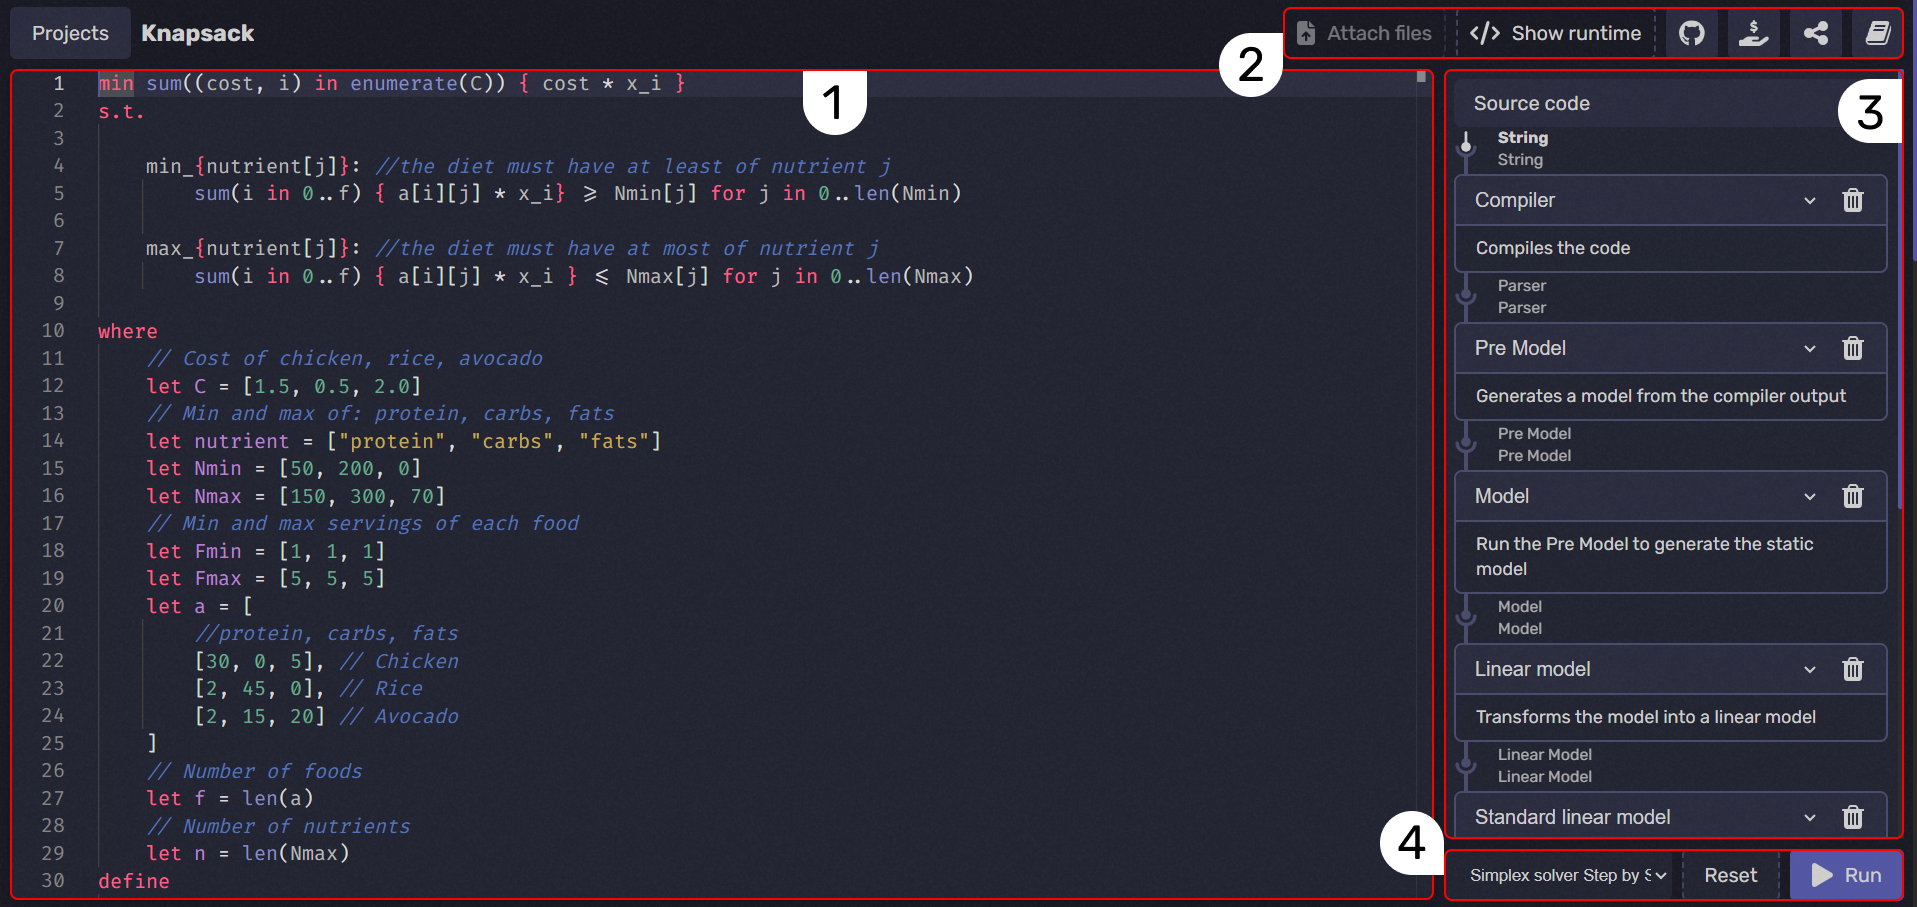
\includegraphics[width=\textwidth]{editor-ui-1.png}%
}{%
  \fbox{\parbox{0.8\textwidth}{\centering Immagine non disponibile}}%
}
\caption{L'editor della piattaforma web: a sinistra l'area di scrittura del
modello, a destra il pannello con la pipeline di risoluzione, configurabile come
sequenza di stadi.}
\label{fig:editor}
\end{figure}

\noindent I riquadri numerati nella Figura~\ref{fig:editor} indicano:
\begin{enumerate}
  \item l'\textbf{editor di codice}, in cui si scrive il modello ROOC (qui il
        problema della dieta dell'Appendice~\ref{app:esempi}), con evidenziazione
        della sintassi e diagnostica in linea;
  \item la \textbf{barra degli strumenti}, con le azioni per allegare file,
        mostrare il \emph{runtime} e accedere al repository, alla condivisione e
        alla documentazione;
  \item il pannello che rappresenta la \emph{pipeline} come
        sequenza di stadi configurabili che l'utente può aggiungere e rimuovere;
  \item i \textbf{controlli di esecuzione}, con la scelta della pipeline
        predefinita e i pulsanti per ripristinare ed eseguire il modello.
\end{enumerate}

\paragraph{Funzionalità da Language Server.}
Sull'editor sono innestate alcune funzionalità tipiche di un \emph{Language
Server Protocol} (LSP), realizzate interamente nel browser appoggiandosi alla
libreria WebAssembly. La segnalazione degli errori sfrutta la diagnostica del
compilatore: gli errori di sintassi, di tipo e di trasformazione, corredati della
loro posizione (Capitoli~\ref{cap:parsing} e~\ref{cap:semantica}), vengono
evidenziati direttamente nel codice. Il passaggio del cursore su un'espressione
ne mostra il tipo, ricavato dalla mappa dei token tipati prodotta dal type
checker (Capitolo~\ref{cap:semantica}). Sono inoltre disponibili il completamento
automatico e la formattazione del codice.

\section{Valore didattico}
\label{sec:valore-didattico}

La caratteristica che distingue la piattaforma è la possibilità di ispezionare
l'intero processo di risoluzione. Come
descritto nel Capitolo~\ref{cap:architettura}, l'architettura a pipe conserva
tutte le rappresentazioni intermedie; la piattaforma le rende visibili, mostrando
il modello dopo l'analisi semantica, la sua resa in LaTeX, la versione
linearizzata, la forma standard e, infine, la risoluzione
(Figura~\ref{fig:output}).

\begin{figure}[H]
\centering
\IfFileExists{imgs/editor-ui-2.png}{%
  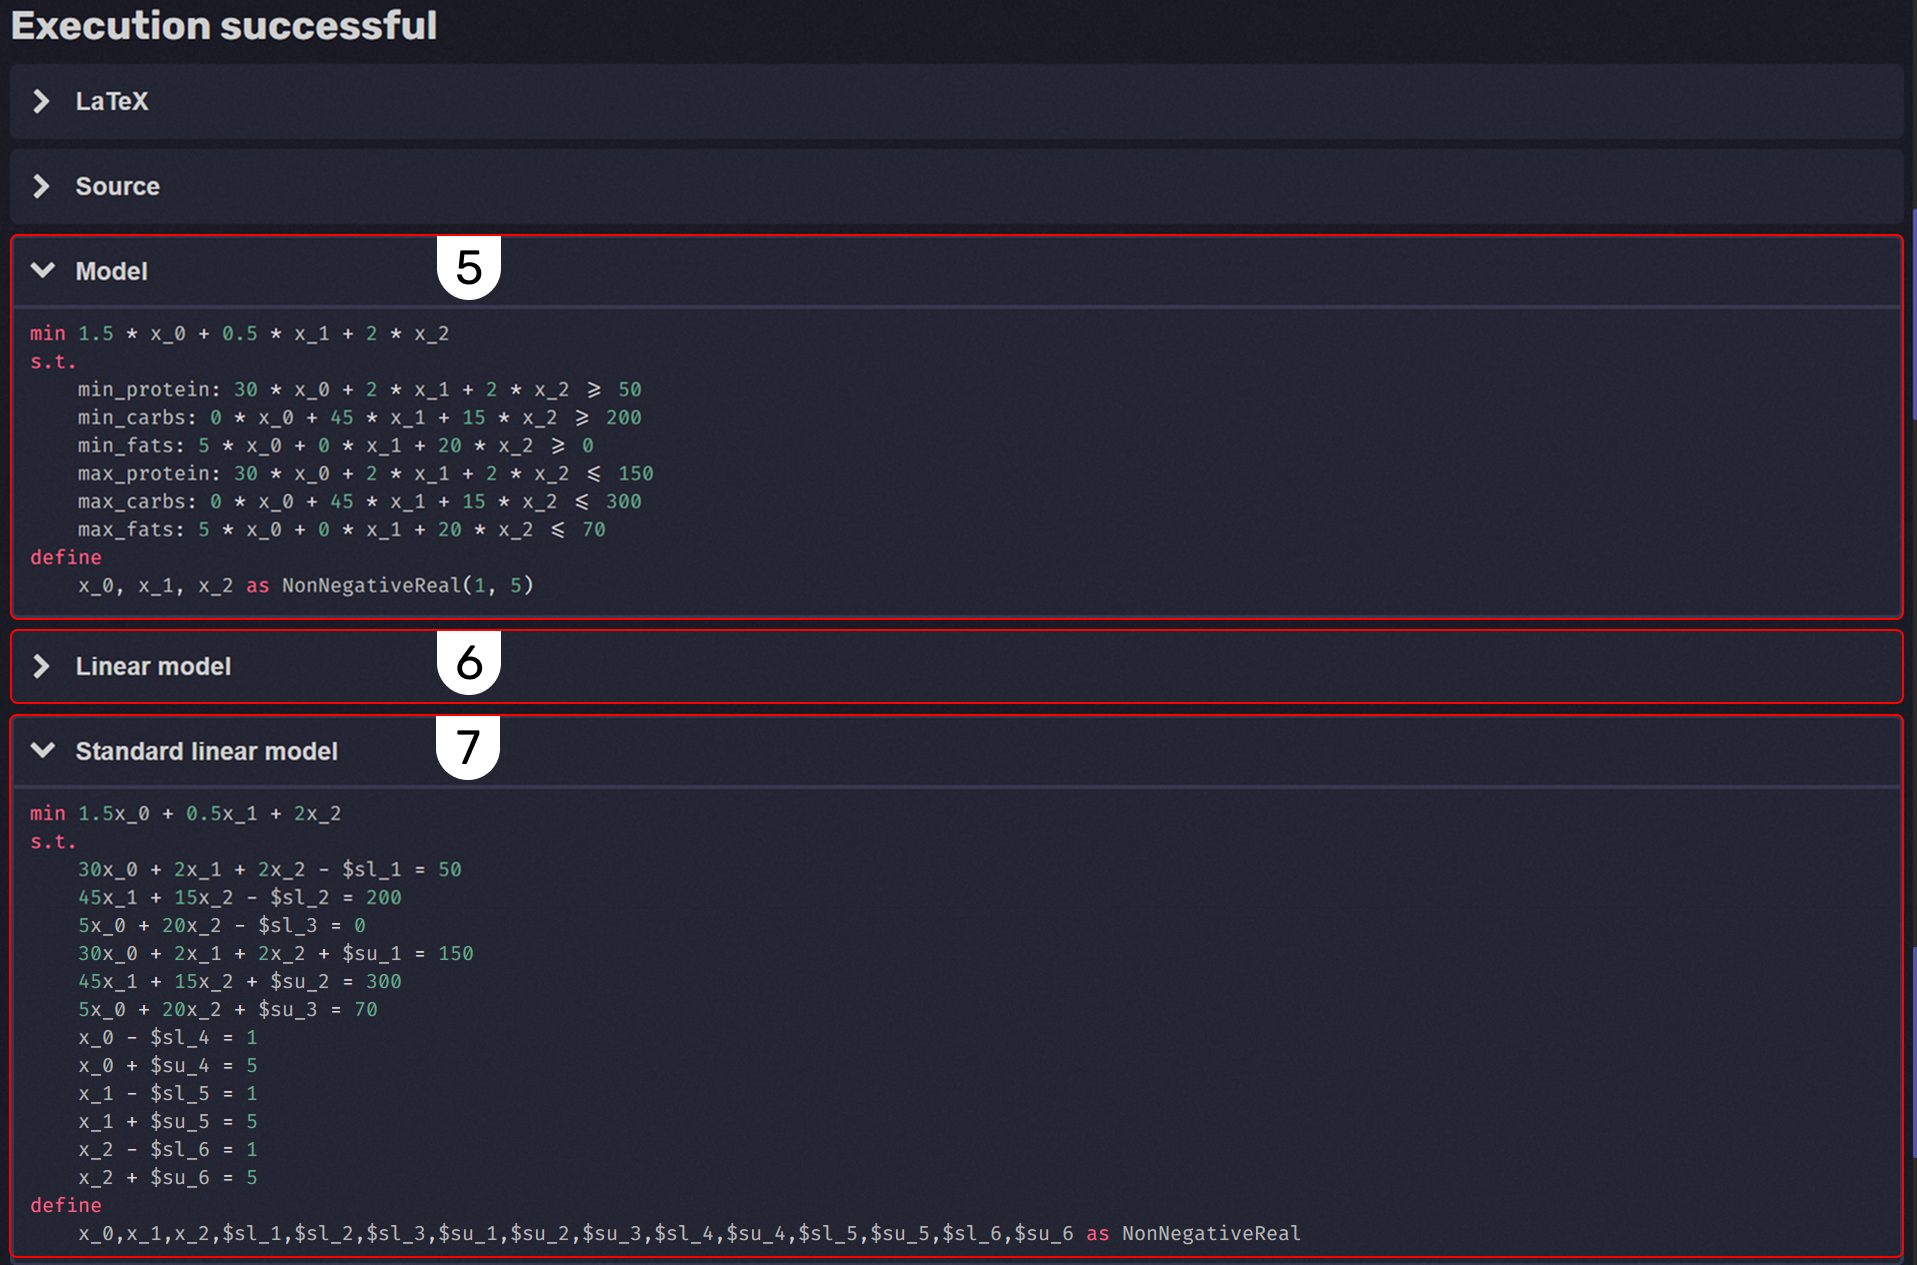
\includegraphics[width=\textwidth]{editor-ui-2.png}%
}{%
  \fbox{\parbox{0.8\textwidth}{\centering Immagine non disponibile}}%
}
\caption{Le rappresentazioni intermedie esposte dopo l'esecuzione, dal modello
alla forma standard.}
\label{fig:output}
\end{figure}

\noindent I riquadri numerati nella Figura~\ref{fig:output} indicano:
\begin{enumerate}
  \setcounter{enumi}{4}
  \item il \textbf{Model}, ottenuto dopo l'analisi semantica
        (Capitolo~\ref{cap:semantica}), in cui le astrazioni di alto livello sono
        risolte: le costanti sono valutate e gli iteratori espansi;
  \item il \textbf{modello lineare}, in cui ogni espressione è ridotta a una
        combinazione lineare delle variabili (qui mostrato compresso dato che già lineare);
  \item il \textbf{modello in forma standard}, con i vincoli ridotti a
        uguaglianze tramite variabili di \emph{slack} e \emph{surplus}, pronto
        per il simplesso.
\end{enumerate}

In particolare, la modalità passo-passo del simplesso (Capitolo~\ref{cap:solver})
permette di osservare l'evoluzione del \emph{tableau} a ogni iterazione, con
l'indicazione delle variabili entrante e uscente
(Figura~\ref{fig:simplex-steps}).

\begin{figure}[H]
\centering
\IfFileExists{imgs/editor-ui-3.png}{%
  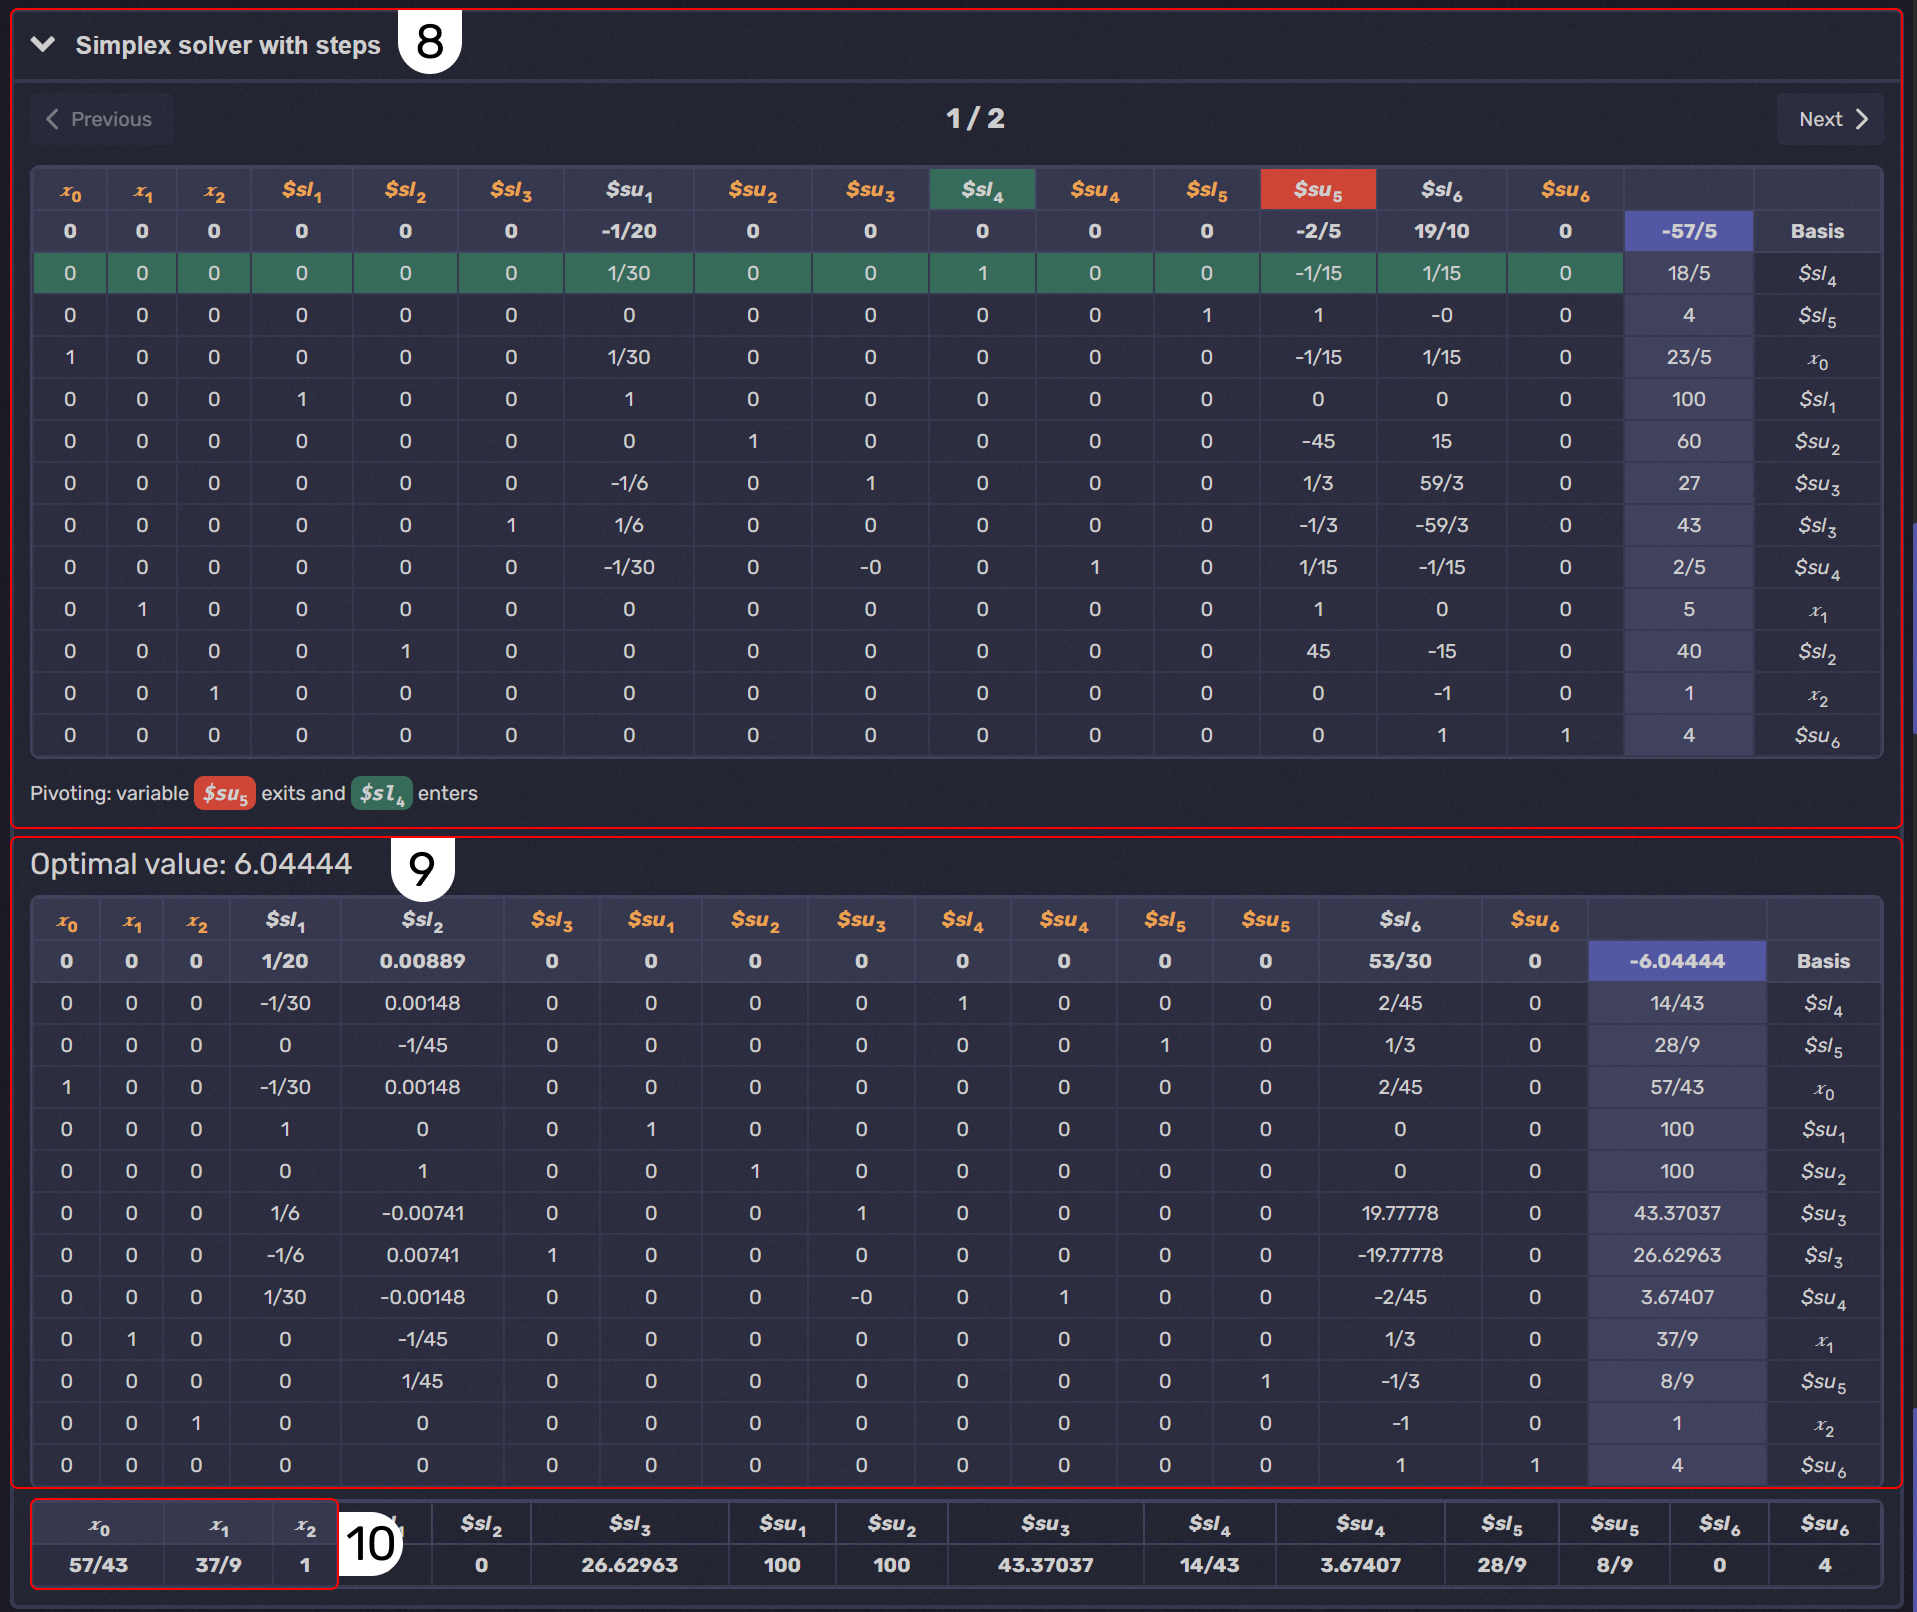
\includegraphics[width=\textwidth]{editor-ui-3.png}%
}{%
  \fbox{\parbox{0.8\textwidth}{\centering Immagine non disponibile}}%
}
\caption{La risoluzione passo-passo del simplesso e la soluzione finale del
problema della dieta.}
\label{fig:simplex-steps}
\end{figure}

\noindent I riquadri numerati nella Figura~\ref{fig:simplex-steps} indicano:
\begin{enumerate}
  \setcounter{enumi}{7}
  \item la \textbf{risoluzione passo-passo} del simplesso, con la navigazione tra
        le iterazioni e l'indicazione, a ogni \emph{pivot}, delle variabili
        entrante e uscente;
  \item il \textbf{tableau ottimo}, raggiunto al termine delle iterazioni, con il
        relativo valore ottimo della funzione obiettivo;
  \item la \textbf{soluzione}, ossia i valori assunti dalle variabili del modello
        (\texttt{x\_0}, \texttt{x\_1}, \texttt{x\_2} e le variabili ausiliarie).
\end{enumerate}

A completamento, la piattaforma offre una documentazione interattiva del
linguaggio, con esempi eseguibili direttamente nell'editor. L'insieme di queste
funzionalità fa sì che ROOC non sia soltanto uno strumento per risolvere modelli
di ottimizzazione, ma anche un mezzo per comprendere come tali modelli vengano
compilati e risolti. In particolare, può essere d'aiuto agli studenti dei corsi
di Ricerca Operativa e di Ottimizzazione Combinatoria, offrendo loro un ambiente
in cui imparare a formulare un modello e a risolverlo con un solver, osservando
al tempo stesso ogni fase del procedimento.

%!TEX root = ../main_thesis.tex

\chapter{Conclusioni e sviluppi futuri}
\label{cap:conclusioni}

\section{Riepilogo dei contributi}
\label{sec:riepilogo}

Questa tesi ha presentato ROOC, un linguaggio per la modellazione di problemi di
ottimizzazione e l'ambiente che lo accompagna. Il lavoro si è concentrato sul
\emph{motore}: un compilatore che traduce un modello, scritto in una notazione
dichiarativa vicina alla matematica, in una forma lineare risolvibile da un
solver.

I contributi principali possono essere riassunti come segue. È stato progettato
un \emph{linguaggio} dotato di un sistema di tipi e di costrutti di alto livello,
come gli iteratori, le \emph{block function}, gli operatori logici e i tipi di
dato strutturati (Capitolo~\ref{cap:linguaggio}). È stato realizzato un \emph{compilatore
multi-fase} che, attraverso una sequenza di trasformazioni
(Capitoli~\ref{cap:parsing}--\ref{cap:linearizzazione}), riduce il modello alla
forma standard, e la cui architettura a \emph{pipe}
(Capitolo~\ref{cap:architettura}) rende ogni fase componibile e ispezionabile. È
stato esteso il solver \texttt{microlp}, a partire da un crate esistente
limitato al simplesso, fino a coprire la programmazione lineare intera mista
(Capitolo~\ref{cap:solver}). Infine, il motore, pure Rust insieme ai suoi
solver predefiniti, è stato reso disponibile come libreria riutilizzabile, anche
attraverso una \emph{fluent API} che porta nell'ecosistema Rust i vincoli logici
nei modelli misti e la loro linearizzazione automatica, e come piattaforma web
didattica
(Capitolo~\ref{cap:piattaforma}).

\section{Limitazioni}
\label{sec:limitazioni}

Il lavoro presenta alcune limitazioni note. Sul piano del linguaggio, gli
operatori logici si applicano soltanto a espressioni booleane: non è possibile
usare un confronto aritmetico come atomo logico (per esempio $(x + y \le 5)
\lor b$), costrutto che richiederebbe la riformulazione dei confronti tramite
costanti \emph{big-M} e quindi un'analisi dei limiti delle variabili. Sul piano
della risoluzione, il simplesso implementato nel
progetto è orientato alla chiarezza didattica più che alle prestazioni, e la sua
applicazione diretta è limitata ai modelli di dimensioni contenute; per i
problemi più impegnativi ci si affida ai solver esterni. Infine, l'intera
pipeline è oggi orientata ai modelli lineari, pur essendo l'architettura
predisposta per ospitare in futuro forme diverse.

\section{Sviluppi futuri}
\label{sec:sviluppi-futuri}

Diversi sono i possibili sviluppi. Il più immediato è l'estensione degli
operatori logici ai confronti aritmetici (\emph{vincoli indicatore}), che
completerebbe la copertura dei problemi di ottimizzazione combinatoria
modellabili in modo diretto. L'architettura a pipe si presta inoltre
all'aggiunta di nuovi solver e di nuove fasi di trasformazione, anche verso
forme non lineari. Sul fronte della piattaforma, l'ulteriore arricchimento degli
strumenti di visualizzazione e della documentazione interattiva ne rafforzerebbe
la vocazione didattica. ROOC si conferma così non solo come uno strumento per
risolvere modelli di ottimizzazione, ma anche come una base estensibile su cui
continuare a costruire.


%   BACK MATTER
%   BIBLIOGRAPHY
\cleardoublepage
\phantomsection
\addcontentsline{toc}{chapter}{\bibname}
\bibliography{refs}

%   APPENDIX
\cleardoublepage
\appendix % to tell LaTeX that the following chapters are appendices
%!TEX root = ../main_thesis.tex

\chapter{Un esempio di compilazione: il problema della dieta}
\label{app:esempi}

Per illustrare in modo concreto l'intera pipeline di compilazione
(Capitolo~\ref{cap:architettura}), si segue qui un singolo modello, il
\emph{problema della dieta}, lungo le sue rappresentazioni intermedie: dal
sorgente al \texttt{Model} prodotto dall'analisi semantica, alla sua versione
lineare (\texttt{LinearModel}) e infine alla forma standard
(\texttt{StandardLinearModel}). Il modello impiega gran parte dei costrutti del
linguaggio descritti nel Capitolo~\ref{cap:linguaggio}: costanti scalari e array
(anche multidimensionali), funzioni della libreria standard (\texttt{enumerate},
\texttt{len}), sommatorie indicizzate, variabili composte, vincoli nominati e
replicati tramite la clausola \texttt{for}, e variabili con estremi dipendenti dai
dati. L'obiettivo è minimizzare il costo complessivo della dieta mantenendo
ciascun nutriente entro i limiti previsti.

\section{Sorgente}
\label{app:diet-sorgente}

Il Listato~\ref{lst:diet} riporta il modello così come viene scritto dall'utente.
I dati dell'istanza (costi, fabbisogni dei nutrienti, porzioni minime e massime e
la matrice \texttt{a} dei valori nutrizionali) sono raccolti nel blocco
\texttt{where}, separati dalla struttura del modello.

\begin{lstlisting}[language=rooc, caption={Il problema della dieta in ROOC.}, label={lst:diet}]
min sum((cost, i) in enumerate(C)) { cost * x_i }
s.t.

    min_{nutrient[j]}: //diet must have at least of nutrient j
        sum(i in 0..f) { a[i][j] * x_i} >= Nmin[j] for j in 0..len(Nmin)

    max_{nutrient[j]}: //diet must have at most of nutrient j
        sum(i in 0..f) { a[i][j] * x_i } <= Nmax[j] for j in 0..len(Nmax)

where
    // Cost of chicken, rice, avocado
    let C = [1.5, 0.5, 2.0]
    // Min and max of: protein, carbs, fats
    let nutrient = ["protein", "carbs", "fats"]
    let Nmin = [50, 200, 0]
    let Nmax = [150, 300, 70]
    // Min and max servings of each food
    let Fmin = [1, 1, 1]
    let Fmax = [5, 5, 5]
    let a = [
        //protein, carbs, fats
        [30, 0, 5], // Chicken
        [2, 45, 0], // Rice
        [2, 15, 20] // Avocado
    ]
    // Number of foods
    let f = len(a)
    // Number of nutrients
    let n = len(Nmax)
define
    //bound the amount of each serving of food i
    x_i as NonNegativeReal(Fmin[i], Fmax[i]) for i in 0..f
\end{lstlisting}

\section{Modello}
\label{app:diet-model}

L'analisi semantica e la trasformazione (Capitolo~\ref{cap:semantica}) producono
il \texttt{Model} del Listato~\ref{lst:diet-model}, in cui tutte le astrazioni di
alto livello sono state risolte. Le costanti sono state valutate e sostituite con
i rispettivi valori; gli iteratori sono stati espansi: la clausola
\texttt{for j in 0..len(Nmin)} replica i vincoli per i tre nutrienti, e il nome
composto \texttt{min\_\{nutrient[j]\}} diventa \texttt{min\_protein},
\texttt{min\_carbs} e \texttt{min\_fats}. Le sommatorie \texttt{sum(i in 0..f)}
sono diventate somme dei tre termini concreti, con i coefficienti letti dalla
matrice \texttt{a}, e le variabili composte \texttt{x\_i} sono state risolte in
\texttt{x\_0}, \texttt{x\_1} e \texttt{x\_2}, ciascuna con dominio
\texttt{NonNegativeReal(1, 5)} (gli estremi \texttt{Fmin[i]} e \texttt{Fmax[i]}
valutati). Si noti che a questo livello possono ancora comparire termini con
coefficiente nullo, come \texttt{0 * x\_0}.

\

\begin{lstlisting}[language=rooc, caption={Il \texttt{Model} dopo l'analisi semantica.}, label={lst:diet-model}]
min 1.5 * x_0 + 0.5 * x_1 + 2 * x_2
s.t.
    min_protein: 30 * x_0 + 2 * x_1 + 2 * x_2 >= 50
    min_carbs: 0 * x_0 + 45 * x_1 + 15 * x_2 >= 200
    min_fats: 5 * x_0 + 0 * x_1 + 20 * x_2 >= 0
    max_protein: 30 * x_0 + 2 * x_1 + 2 * x_2 <= 150
    max_carbs: 0 * x_0 + 45 * x_1 + 15 * x_2 <= 300
    max_fats: 5 * x_0 + 0 * x_1 + 20 * x_2 <= 70
define
    x_0, x_1, x_2 as NonNegativeReal(1, 5)
\end{lstlisting}

\section{Modello lineare}
\label{app:diet-linear}

La linearizzazione (Capitolo~\ref{cap:linearizzazione}) riduce ogni espressione a
una combinazione lineare delle variabili. I termini con coefficiente nullo vengono
eliminati (per esempio \texttt{0 * x\_0} scompare da \texttt{min\_carbs} e
\texttt{0 * x\_1} da \texttt{min\_fats}) e si adotta la moltiplicazione implicita.
Il risultato è il \texttt{LinearModel} del Listato~\ref{lst:diet-linear}, in cui
restano soltanto le variabili effettivamente utilizzate in ciascun vincolo.

\begin{lstlisting}[language=rooc, caption={Il \texttt{LinearModel} dopo la linearizzazione.}, label={lst:diet-linear}]
min 1.5x_0 + 0.5x_1 + 2x_2
s.t.
    min_protein: 30x_0 + 2x_1 + 2x_2 >= 50
    min_carbs: 45x_1 + 15x_2 >= 200
    min_fats: 5x_0 + 20x_2 >= 0
    max_protein: 30x_0 + 2x_1 + 2x_2 <= 150
    max_carbs: 45x_1 + 15x_2 <= 300
    max_fats: 5x_0 + 20x_2 <= 70
define
    x_0, x_1, x_2 as NonNegativeReal(1, 5)
\end{lstlisting}

\section{Forma standard}
\label{app:diet-standard}

L'ultima trasformazione (Sezione~\ref{sec:forma-standard}) riduce il modello alla
forma standard del Listato~\ref{lst:diet-standard}, richiesta dal simplesso. Ogni
disuguaglianza diventa un'uguaglianza con l'aggiunta di una variabile non
negativa: una variabile sottratta per i vincoli di tipo \texttt{>=} e una aggiunta
per quelli di tipo \texttt{<=} (qui con i nomi generati automaticamente
\texttt{\$sl\_k} e \texttt{\$su\_k}). Inoltre gli estremi di ciascuna variabile,
prima espressi dal dominio \texttt{NonNegativeReal(1, 5)}, diventano due vincoli
espliciti (\texttt{>= 1} e \texttt{<= 5}), a loro volta normalizzati a uguaglianze.
Poiché l'obiettivo era già di minimizzazione, non viene negato.

\begin{lstlisting}[language=rooc, caption={Il modello in forma standard.}, label={lst:diet-standard}]
min 1.5x_0 + 0.5x_1 + 2x_2
s.t.
    30x_0 + 2x_1 + 2x_2 - $sl_1 = 50
    45x_1 + 15x_2 - $sl_2 = 200
    5x_0 + 20x_2 - $sl_3 = 0
    30x_0 + 2x_1 + 2x_2 + $su_1 = 150
    45x_1 + 15x_2 + $su_2 = 300
    5x_0 + 20x_2 + $su_3 = 70
    x_0 - $sl_4 = 1
    x_0 + $su_4 = 5
    x_1 - $sl_5 = 1
    x_1 + $su_5 = 5
    x_2 - $sl_6 = 1
    x_2 + $su_6 = 5
\end{lstlisting}


%   ACKNOWLEDGEMENTS
% \cleardoublepage
% \pagenumbering{gobble}
% \thispagestyle{plain}			% Supress header
\section*{Ringraziamenti}
Vorrei ringraziare il Prof. Matteo Spezialetti, il Prof. Stefano Smriglio, il Prof. Luca Forlizzi e il Prof. Claudio Arbib per i loro insegnamenti, che hanno alimentato la mia curiosità e la mia passione per l'informatica.

I miei genitori, mia sorella e la mia famiglia, per il loro supporto e incoraggiamento durante tutto il mio percorso di studi.

I miei amici e colleghi, per tutto il divertimento, per aver condiviso con me i loro interessi e per avermi mostrato prospettive e opportunità che altrimenti non avrei mai considerato.

I miei coinquilini, per tutte le giornate trascorse insieme, le cene condivise e le birre bevute.

\bigskip

\emph{Addio, e grazie per tutto il pesce.}

\vspace{1.5cm}
\hfill
Enrico Menichelli, L'Aquila, Ottobre 2026

\newpage				% Create empty back of side
\thispagestyle{empty}
\mbox{}

\end{document}
